\clearpage
\section{Device examples}
\subsection{An axisymmetric disk model}
\begin{flushleft}
  \textbf{Inputfile:}
  \ttt{\ttilde/hiqlab/models/developing/disk\_resonator/disk\_new}\\
  \textbf{Lua functions used:}
\end{flushleft}

\begin{figure}[htbp]
\centering
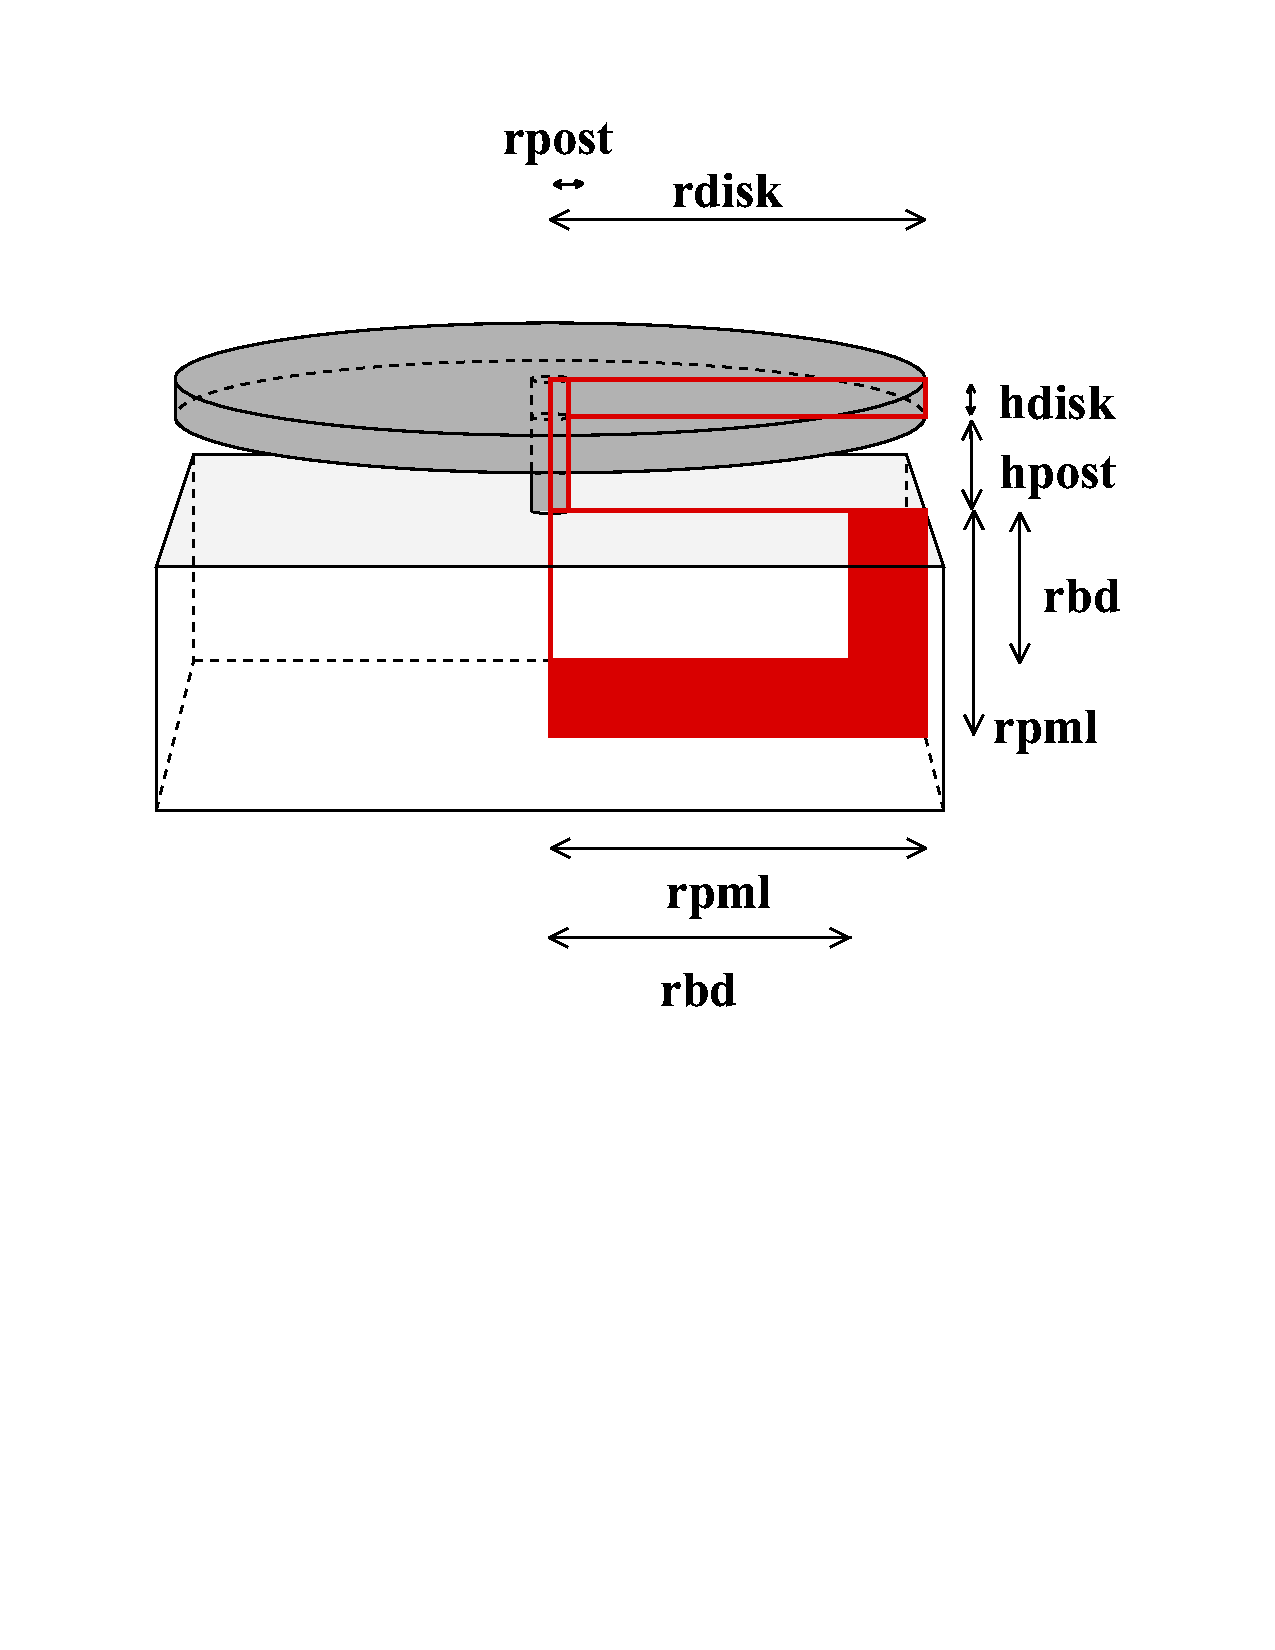
\includegraphics[trim = 0in 4in 0.1in 0in, clip, height = 3in]{fig/disk_resonator.pdf}
\caption{Schematic of the Disk resonator}
\label{fig:DiskResonator}
\end{figure}

\clearpage
\subsubsection*{Input file (LUA)}
\begin{flushleft}
  \textbf{Inputfile:}
  \ttt{\ttilde/hiqlab/models/developing/disk\_resonator/disk\_new/disk\_mesh.lua}\\
\end{flushleft}
\hspace{1in}
{\footnotesize
\listinginput[10]{1}{../../../models/developing/disk_resonator/disk_new/diskmesh.lua}
}

\clearpage
Only the portions emphasized are explained in detail.

\begin{itemize}

  \item{\textbf{Define element type:}}
  Two types of elastic material are defined, for modeling the 
  case where the post and disk material differ.

  \item{\textbf{Define driving and sensing functions:}}
  The disk is driven by a radial force at the perimeter and 
  sensed at the same location.

\end{itemize}

\clearpage
\subsubsection*{Solve dynamic modal problem (MATLAB)}
\begin{flushleft}
  \textbf{Inputfile:}
  \ttt{\ttilde/hiqlab/models/developing/disk\_resonator/disk\_new/disk\_dyn.m}\\
\end{flushleft}
\hspace{1in}
{\footnotesize
\listinginput[10]{1}{../../../models/developing/disk_resonator/disk_new/disk_dyn.m}
}

\clearpage
The steps to compute the dynamic modes of the disk resonator are 
explained here. 

\begin{itemize}

  \item{\textbf{Compute frequencies, Qs, and mode shapes:}}
  The function \ttt{mechmode} is used to compute \ttt{nev}
  modes closest to the frequence \ttt{w0}[rad/s]. The frequencies
  are sorted from proximity to \ttt{w0}.

  \item{\textbf{Show modes obtained:}}
  \ttt{plot\_mode} displays the obtained modes. Several options
  can be passed. In this case, the modes are animated by
  the \ttt{opt.animate} option which calls \ttt{plot\_cycle2d}. 

\end{itemize}

The modal values obtained for this problem are,
\begin{verbatim}
Freq [Hz]   :2.888937e+08
            :1.030763e+05
Q           :1.401359e+03
\end{verbatim}

\begin{figure}[htbp]
\centering
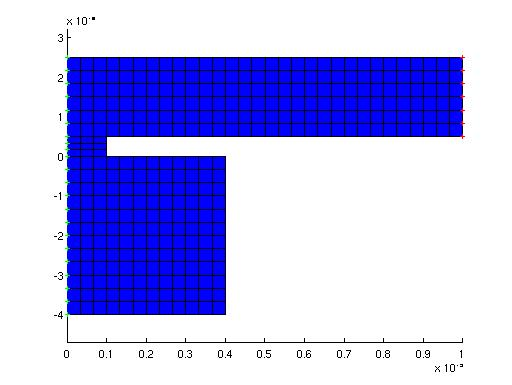
\includegraphics[height = 3in]{fig/disk_resonator_mesh.jpg}
\caption{Mesh of disk resonator}
\label{fig:DiskResonatorMesh}
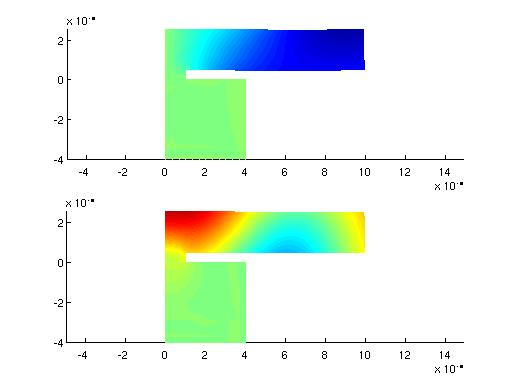
\includegraphics[height = 3in]{fig/disk_resonator_mode.jpg}
\caption{Mode of disk resonator}
\label{fig:DiskResonatorMode}
\end{figure}

\clearpage
\subsubsection*{Solve for forced response (MATLAB)}
\begin{flushleft}
  \textbf{Inputfile:}
  \ttt{\ttilde/hiqlab/models/developing/disk\_resonator/disk\_new/disk\_for.m}\\
\end{flushleft}
\hspace{1in}
{\footnotesize
\listinginput[10]{1}{../../../models/developing/disk_resonator/disk_new/disk_for.m}
}

\clearpage
The steps to compute the dynamic response to a time harmonic
force of the disk resonator are explained here. 

\begin{itemize}

  \item{\textbf{Form driving pattern and obtain harmonic response:}}
  The driving pattern is obtained by \ttt{Mesh\_get\_drive\_f}
  which looks for the function \ttt{bode\_drive\_function} in 
  the Lua input file. Along with this driving pattern the 
  forcing frequency \ttt{w}[rad/s] is given to the 
  \ttt{harmonic\_state}.

\end{itemize}

\clearpage
\subsubsection*{Solve for transfer function (MATLAB)}
\begin{flushleft}
  \textbf{Inputfile:}
  \ttt{\ttilde/hiqlab/models/developing/disk\_resonator/disk\_new/disk\_tra.m}\\
\end{flushleft}
\hspace{1in}
{\footnotesize
\listinginput[10]{1}{../../../models/developing/disk_resonator/disk_new/disk_tra.m}
}

\clearpage
The steps to compute the transfer function of the disk 
resonator are explained here. 

\begin{itemize}

  \item{\textbf{Form driving and sensing pattern:}}
  These are obtained by calling the functions 
  \ttt{Mesh\_get\_drive\_f} and \ttt{Mesh\_get\_sense\_u}
  which in turn look for the functions 
  \ttt{bode\_drive\_function} and \ttt{bode\_sense\_function}
  in the Lua input file.

  \item{\textbf{Computing transfer function:}}
  \ttt{second\_order\_bode} computes the transfer function
  of a second order system. The transfer function in the
  range of [\ttt{wr\_min*wc},\ttt{wr\_max*wc}] with \ttt{w\_ndiv}
  data points is computed. Optionally, a reduced order model (ROM) 
  can be formed to speed the computation. This is done by 
  specifying the \ttt{kmax} option which defines the size
  of the ROM. In the PML case, a real basis
  can be selected for projection by the option \ttt{realbasis}.
  This option will double the size of the ROM.
 
  \item{\textbf{Show bode plot:}}
  The option \ttt{visualQ} computes and displays the Q value 
  computed from the data points. Enough data points are requred
  for an accurate value.  

\end{itemize}

\begin{figure}[htbp]
\centering
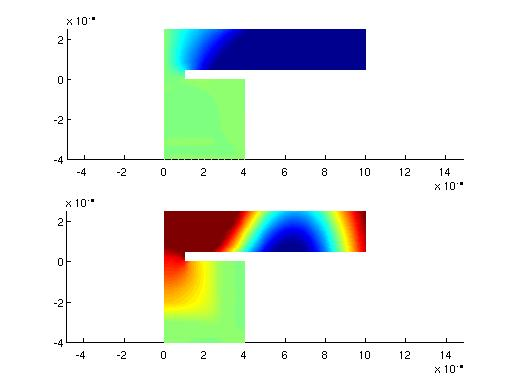
\includegraphics[height = 3in]{fig/disk_resonator_forced.jpg}
\caption{Forced response of disk resonator}
\label{fig:DiskResonatorForced}
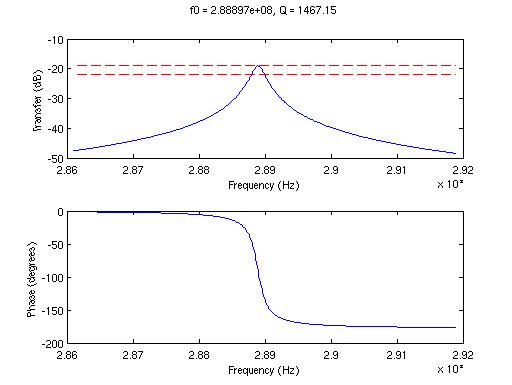
\includegraphics[height = 3in]{fig/disk_resonator_transfer.jpg}
\caption{Transfer function  of disk resonator}
\label{fig:DiskResonatorTransfer}
\end{figure}

\clearpage
\subsection{Michigan Free-Free beam}
\begin{flushleft}
  \textbf{Inputfile:}
  \ttt{\ttilde/hiqlab/models/developing/mich\_la\_fr\_beam}\\
  \textbf{Lua functions used:}
\end{flushleft}

\begin{figure}[htbp]
\centering
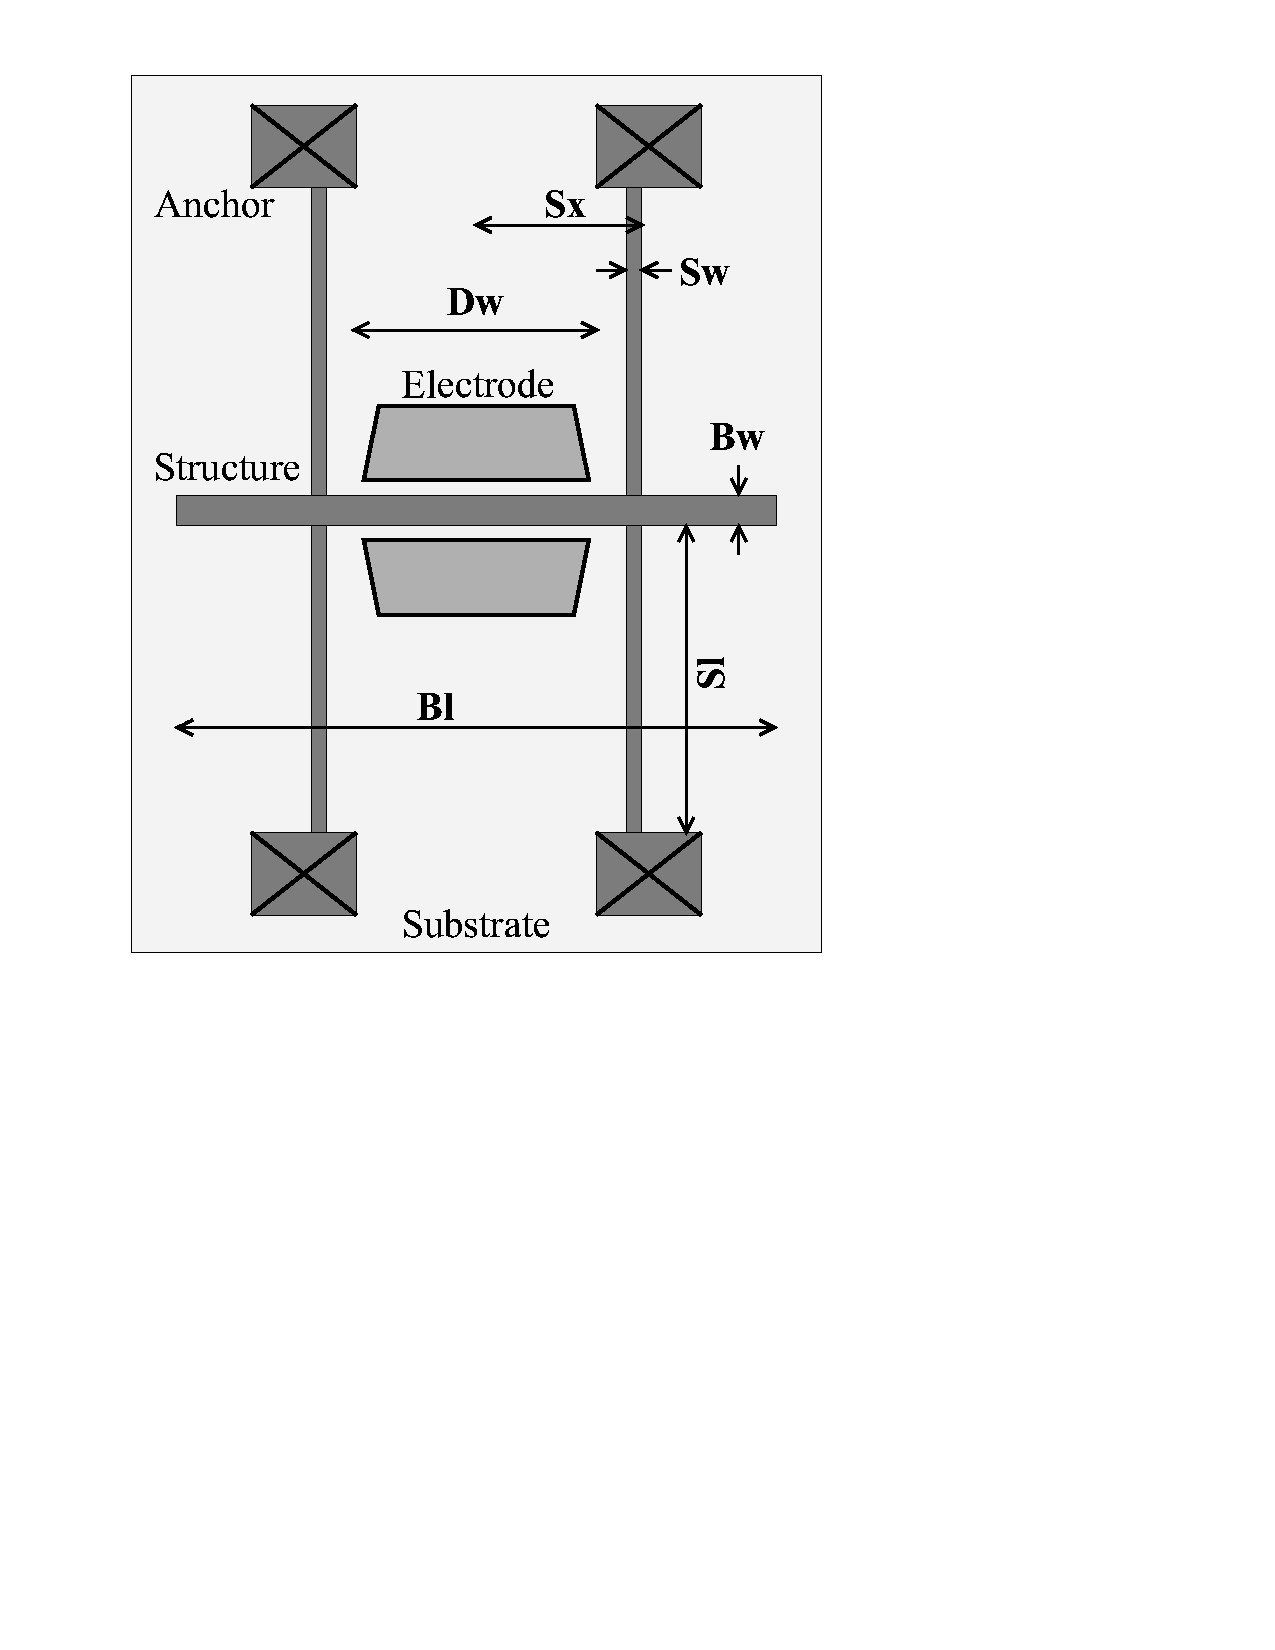
\includegraphics[trim = 0in 4in 1in 0in, clip, height = 3in]{fig/mich_la_frfr_beam2d_small.pdf}
\caption{Schematic of the Michigan Beam Resonator}
\label{fig:MichiganBeamResonator}
\end{figure}

\clearpage
\subsubsection*{Input file (LUA)}
\begin{flushleft}
  \textbf{Inputfile:}
  \ttt{\ttilde/hiqlab/models/developing/mich\_la\_fr\_beam/2d/mich\_la\_frfr\_beam2d.lua}\\
\end{flushleft}
\hspace{1in}
{\footnotesize
\listinginput[10]{1}{../../../models/developing/mich_la_fr_beam/2d/mich_la_frfr_beam2d.lua}
}

\clearpage
Only the portions emphasized are explained in detail.

\begin{itemize}

  \item{\textbf{Including function definition file:}}
  When the mesh generation of a particular geometry becomes
  complex, it is often useful to construct a seperate Lua
  file and include this by calling \ttt{require}. In this
  case \ttt{generate\_frfr\_beam2d.lua} is called.

  \item{\textbf{Define nondimensionalization parameters:}}
  The material \ttt{silicon2} and the length scale of 
  \ttt{2d-6} are used to define the characteristic parameters
  for the thermoelastic analysis through the function 
  \ttt{ted\_nondim}.

  \item{\textbf{Generate Free-Free beam:}}
  The function \ttt{generate\_frfr\_beam2d} is called from
  the file \ttt{generate\_frfr\_beam2d.lua}. The input
  arguments define the location and angle of rotation of the
  device in global coordinates. The function returns a table 
  of functions which define the boundary condition and stretch
  functions of the anchor.  

\end{itemize}

\clearpage
\subsubsection*{Solve dynamic modal problem (MATLAB)}
\begin{flushleft}
  \textbf{Inputfile:}
  \ttt{\ttilde/hiqlab/models/developing/mich\_la\_fr\_beam/2d/mich\_la\_frfr\_beam2d\_dyn.m}\\
\end{flushleft}
\hspace{1in}
{\footnotesize
\listinginput[10]{1}{../../../models/developing/mich_la_fr_beam/2d/mich_la_frfr_beam2d_dyn.m}
}

\clearpage
The steps to compute the dynamic modes of the disk resonator are 
explained here. 

\begin{itemize}

  \item{\textbf{Compute frequencies, Qs, and mode shapes:}}
  The function \ttt{tedmode} is used to compute \ttt{nev}
  modes closest to the frequence \ttt{w0}[rad/s]. 

  \item{\textbf{Show modes obtained:}}
  \ttt{plot\_mode} displays the obtained modes. Several options
  can be passed. In this case, the modes are animated by
  the \ttt{opt.animate} option which calls \ttt{plot\_cycle2d}. 
  Also \ttt{cfields} is specified to show the thermal fluctuations
  for the color field.

\end{itemize}

The modal values obtained are,
\begin{verbatim}
Freq [Hz]   :9.592613e+06
            :3.572215e+02
Q           :1.342670e+04
\end{verbatim}

\begin{figure}[htbp]
\centering
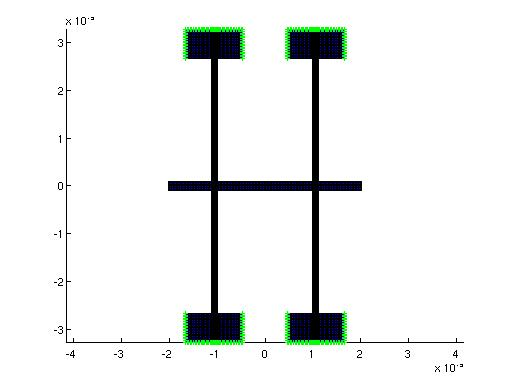
\includegraphics[height = 3in]{fig/mich_resonator_mesh.jpg}
\caption{Mesh of the beam resonator}
\label{fig:MichResonatorMesh}
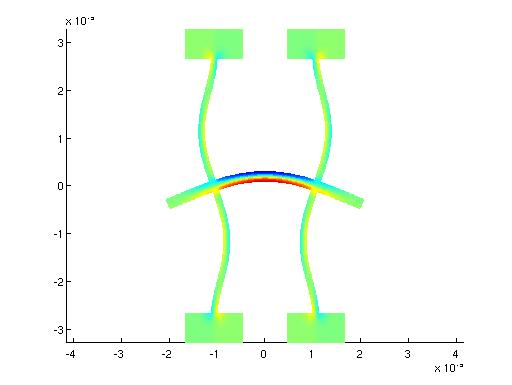
\includegraphics[height = 3in]{fig/mich_resonator_mode.jpg}
\caption{Mode of the beam resonator}
\label{fig:MichResonatorMode}
\end{figure}

\clearpage
\subsubsection*{Solve dynamic forced problem (MATLAB)}
\begin{flushleft}
  \textbf{Inputfile:}
  \ttt{\ttilde/hiqlab/models/developing/mich\_la\_fr\_beam/2d/mich\_la\_frfr\_beam2d\_for.m}\\
\end{flushleft}
\hspace{1in}
{\footnotesize
\listinginput[10]{1}{../../../models/developing/mich_la_fr_beam/2d/mich_la_frfr_beam2d_for.m}
}

\clearpage
The steps to compute the dynamic response to a time harmonic
force of the beam resonator are explained here. 

\begin{itemize}

  \item{\textbf{Form driving pattern and obtain harmonic response:}}
  The driving pattern is obtained by \ttt{Mesh\_get\_drive\_f}
  which looks for the function \ttt{bode\_drive\_function} in 
  the Lua input file. Along with this driving pattern the 
  forcing frequency \ttt{w}[rad/s] is given to the 
  \ttt{harmonic\_state}. The option \ttt{mkc} is set to one
  specifying that the damping term \ttt{C} be included in the 
  computation. This must be specified for the thermoelastic 
  case. 

\end{itemize}

\clearpage
\subsubsection*{Solve transfer function problem (MATLAB)}
\begin{flushleft}
  \textbf{Inputfile:}
  \ttt{\ttilde/hiqlab/models/developing/mich\_la\_fr\_beam/2d/mich\_la\_frfr\_beam2d\_tra.m}\\
\end{flushleft}
\hspace{1in}
{\footnotesize
\listinginput[10]{1}{../../../models/developing/mich_la_fr_beam/2d/mich_la_frfr_beam2d_tra.m}
}

\clearpage
The steps to compute the transfer function of the disk
resonator are explained here. 

\begin{itemize}

  \item{\textbf{Form driving and sensing pattern:}}
  These are obtained by calling the functions
  \ttt{Mesh\_get\_drive\_f} and \ttt{Mesh\_get\_sense\_u}
  which in turn look for the functions
  \ttt{bode\_drive\_function} and \ttt{bode\_sense\_function}
  in the Lua input file.

  \item{\textbf{Computing transfer function:}}
  \ttt{second\_order\_bode} computes the transfer function
  of a second order system. The transfer function in the
  range of [\ttt{wr\_min*wc},\ttt{wr\_max*wc}] with \ttt{w\_ndiv}
  data points is computed. The option \ttt{mkc} is set to one
  specifying that the damping term \ttt{C} be included in the 
  computation. This must be specified for the thermoelastic 
  case. Optionally, a reduced order model (ROM)
  can be formed to speed the computation. This is done by
  specifying the \ttt{kmax} option which defines the size
  of the ROM. In the PML case, a real basis
  can be selected for projection by the option \ttt{realbasis}.
  This option will double the size of the ROM. For the 
  thermoelastic case an additional strucutre preseravation
  basis can be selected by \ttt{structurep}. To do this
  the function \ttt{ted\_block\_mesh} which reorders the 
  \ttt{id} array into mechanical and thermal must be called
  after \ttt{Mesh\_load} as is done in this example.
  This option will double the size of the ROM. 

\end{itemize}

\begin{figure}[htbp]
\centering
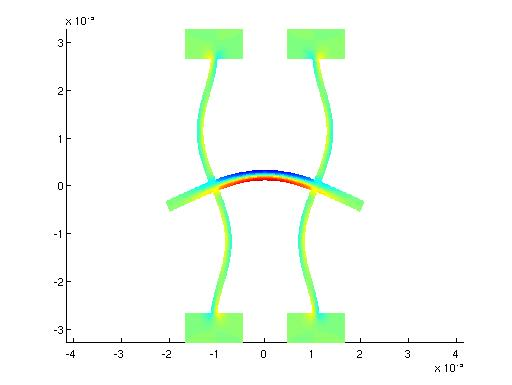
\includegraphics[height = 3in]{fig/mich_resonator_forced.jpg}
\caption{Forced response of Michigan resonator}
\label{fig:MichResonatorForced}
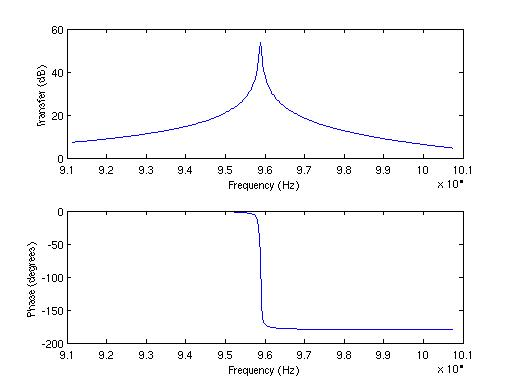
\includegraphics[height = 3in]{fig/mich_resonator_transfer.jpg}
\caption{Transfer function  of Michigan resonator}
\label{fig:MichResonatorTransfer}
\end{figure}

\clearpage
\subsection{Circuit test}
\subsubsection{Low pass filter}
\begin{flushleft}
  \textbf{Inputfile:}
  \ttt{\ttilde/hiqlab/models/tutorial/circuit\_test}\\
  \textbf{Lua functions used:}
\end{flushleft}

\begin{figure}[htbp]
\centering
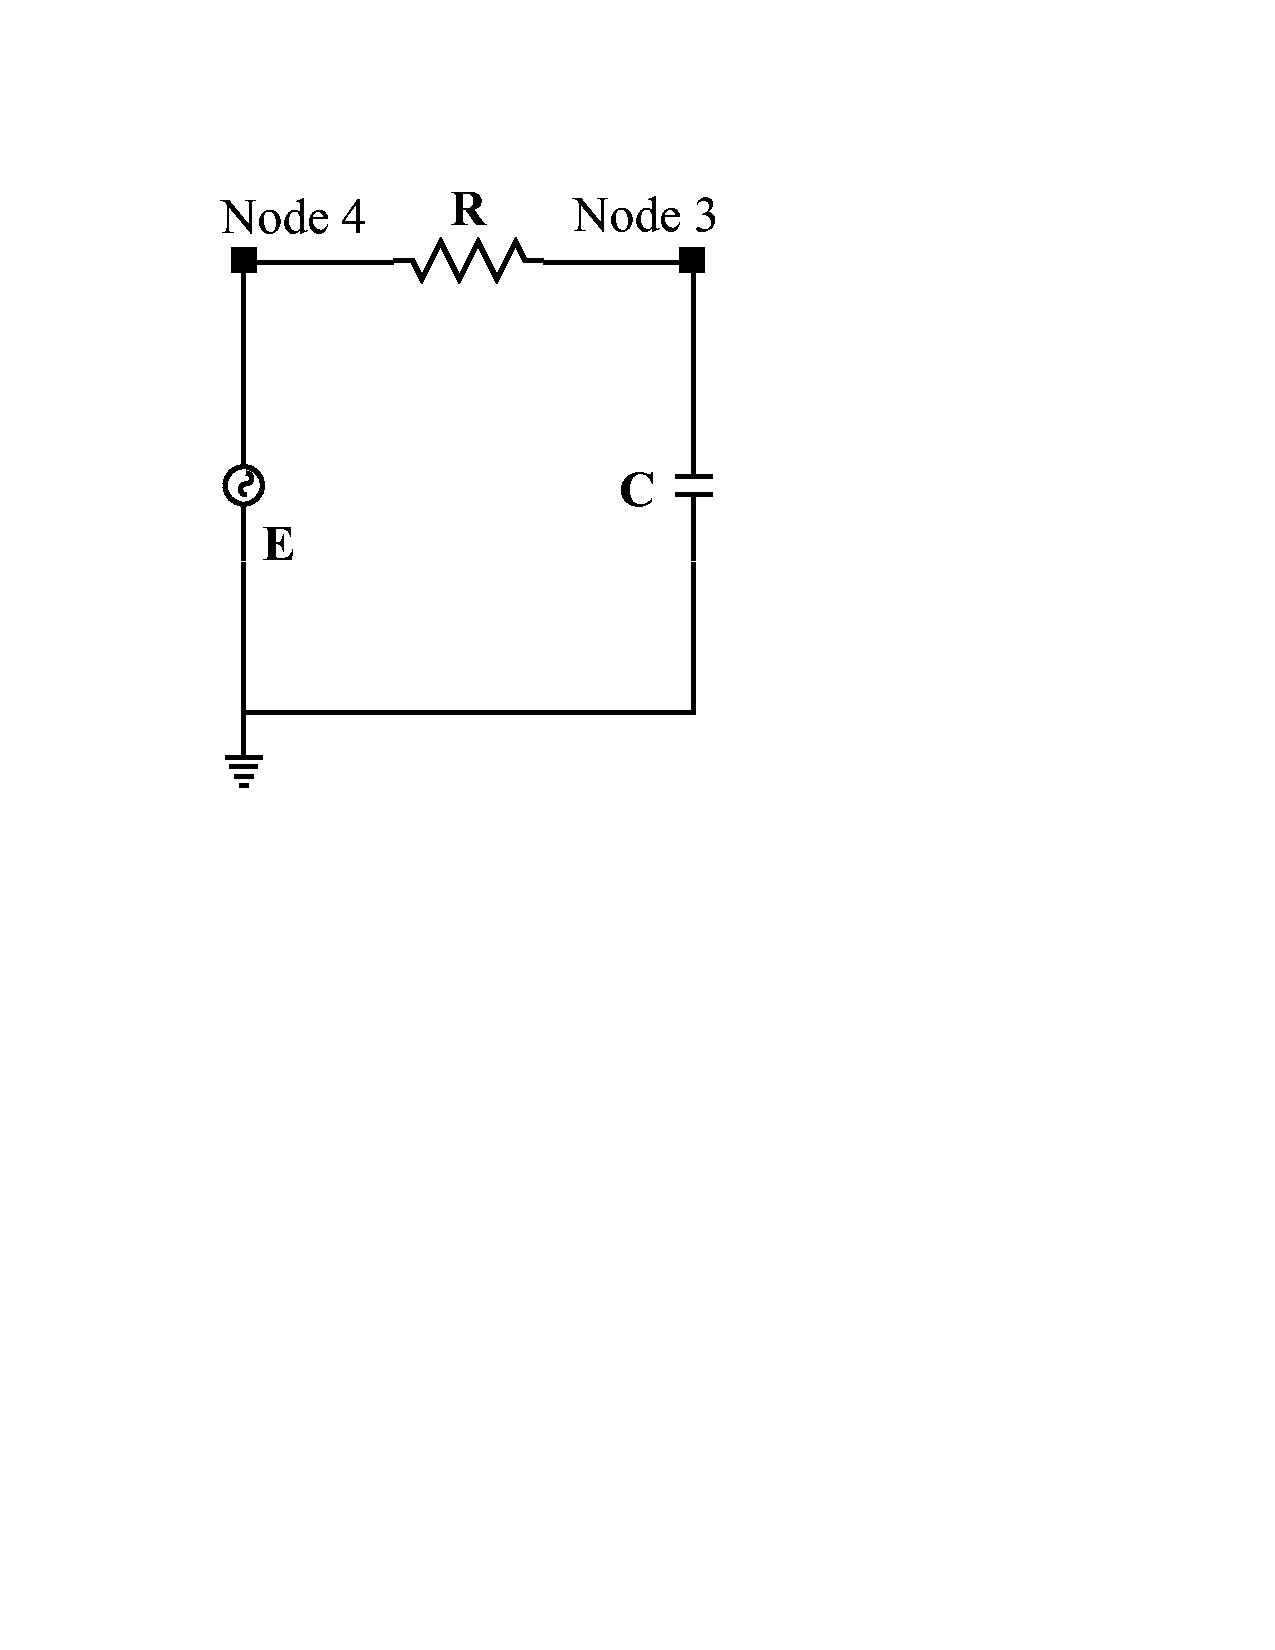
\includegraphics[trim = 0in 5in 1in 1in, clip, height = 3in]{fig/lowpassfilter.pdf}
\caption{Schematic of the Low pass filter}
\label{fig:LowPassFilter}
\end{figure}

\clearpage
\subsubsection*{Input file (LUA)}
\begin{flushleft}
  \textbf{Inputfile:}
  \ttt{\ttilde/hiqlab/models/tutorial/circuit\_test/low\_pass\_filter.lua}\\
\end{flushleft}
\hspace{1in}
{\footnotesize
\listinginput[10]{1}{../../../models/tutorial/circuit_test/low_pass_filter.lua}
}

\clearpage
Only the portions emphasized are explained in detail.

\begin{itemize}

  \item{\textbf{Construct element:}}
  \ttt{make\_material\_LRC} constructs the lumped LRC component
  models used in circuit analysis. The first argument specifies
  the value of the element, and the second the type of component.
  \ttt{make\_material\_wire} constructs an element which 
  can be used for a short circuited wire and additionaly 
  voltage or current sources depending on the element variable 
  boundary conditions that are set.

  \item{\textbf{Add elements to mesh:}}
  The lumped LRC elements are connected between two nodes
  with appropriate node numbers. Since we would like to specify
  a voltage source on the \ttt{wire} element through an element
  variable boundary condition, the element number \ttt{elem1}
  must be extracted and stored for reference.

  \item{\textbf{Define nodal boundary condition:}}
  The nodes which are grounded are specified.

  \item{\textbf{Define driving and sensing functions:}}
  The circuit is driven with an AC voltage source defined 
  through an element variable driving condition on the 
  \ttt{wire} element by the function \ttt{ac\_voltage\_source}. 
  If the index of the
  element \ttt{ind} equals the element number \ttt{elem1} of
  the wire, a value of \ttt{E} is specfied as the voltage
  difference between the nodes that \ttt{wire} is connected to. 

  The voltages at node 3 an 4 are sensed. 

\end{itemize}

\clearpage
\subsubsection*{Solve for transfer function (MATLAB)}
\begin{flushleft}
  \textbf{Inputfile:}
  \ttt{\ttilde/hiqlab/models/tutorial/circuit\_test/low\_pass\_filter.m}\\
\end{flushleft}
\hspace{1in}
{\footnotesize
\listinginput[10]{1}{../../../models/tutorial/circuit_test/low_pass_filter.m}
}

\clearpage
The steps to compute the transfer function of the low pass
filter are explained here. 

\begin{itemize}

  \item{\textbf{Get driving and sensing patterns:}}
  The sensing patterns for the voltages at node 3 and 4
  are obtained by the function \ttt{Mesh\_get\_sense\_u}
  which in turn look for the appropriate functions in the
  Lua input file. Since the driving pattern is obtained
  by the contribution that comes from an element variable
  in \ttt{wire} defined by the Lua function 
  \ttt{ac\_voltage\_source}, it must be called by 
  \ttt{Mesh\_get\_drive\_elements\_f}.

  \item{\textbf{Compute transfer function:}}
  The frequency range can also be set in a logarthmic
  spacing by the option \ttt{w\_type}. In this case
  the range is set as [\ttt{10\^(-2)*wc,10\^(3)*wc}]
  with \ttt{w\_ndiv} divisions. Though this is a first
  order problem the function second order bode can be 
  called for transfer function evaluation, but the 
  option  \ttt{mkc} must be set to 1 to include the 
  \ttt{C} matrix.

\end{itemize}

\begin{figure}[htbp]
\centering
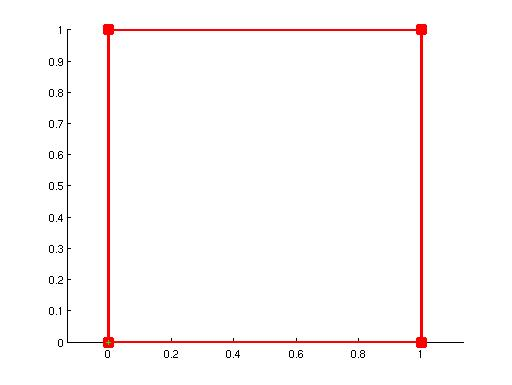
\includegraphics[height = 3in]{fig/low_pass_filter_mesh.jpg}
\caption{Mesh for a Low pass filter}
\label{fig:LowPassFilterMesh}
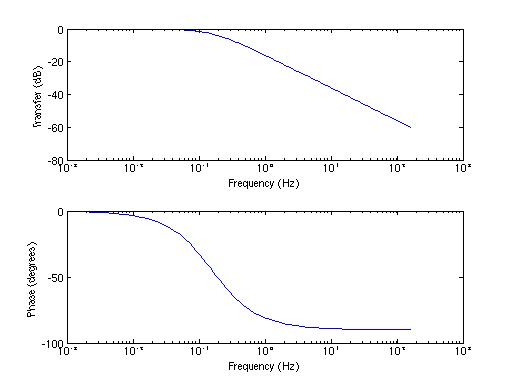
\includegraphics[height = 3in]{fig/low_pass_filter_transfer.jpg}
\caption{Transfer function  for a Low pass filter}
\label{fig:LowPassFilterTransfer}
\end{figure}

\clearpage
\subsubsection{Ladder filter}
\begin{flushleft}
  \textbf{Inputfile:}
  \ttt{\ttilde/hiqlab/models/developing/circuit\_test}\\
  \textbf{Lua functions used:}
\end{flushleft}

\begin{figure}[htbp]
\centering
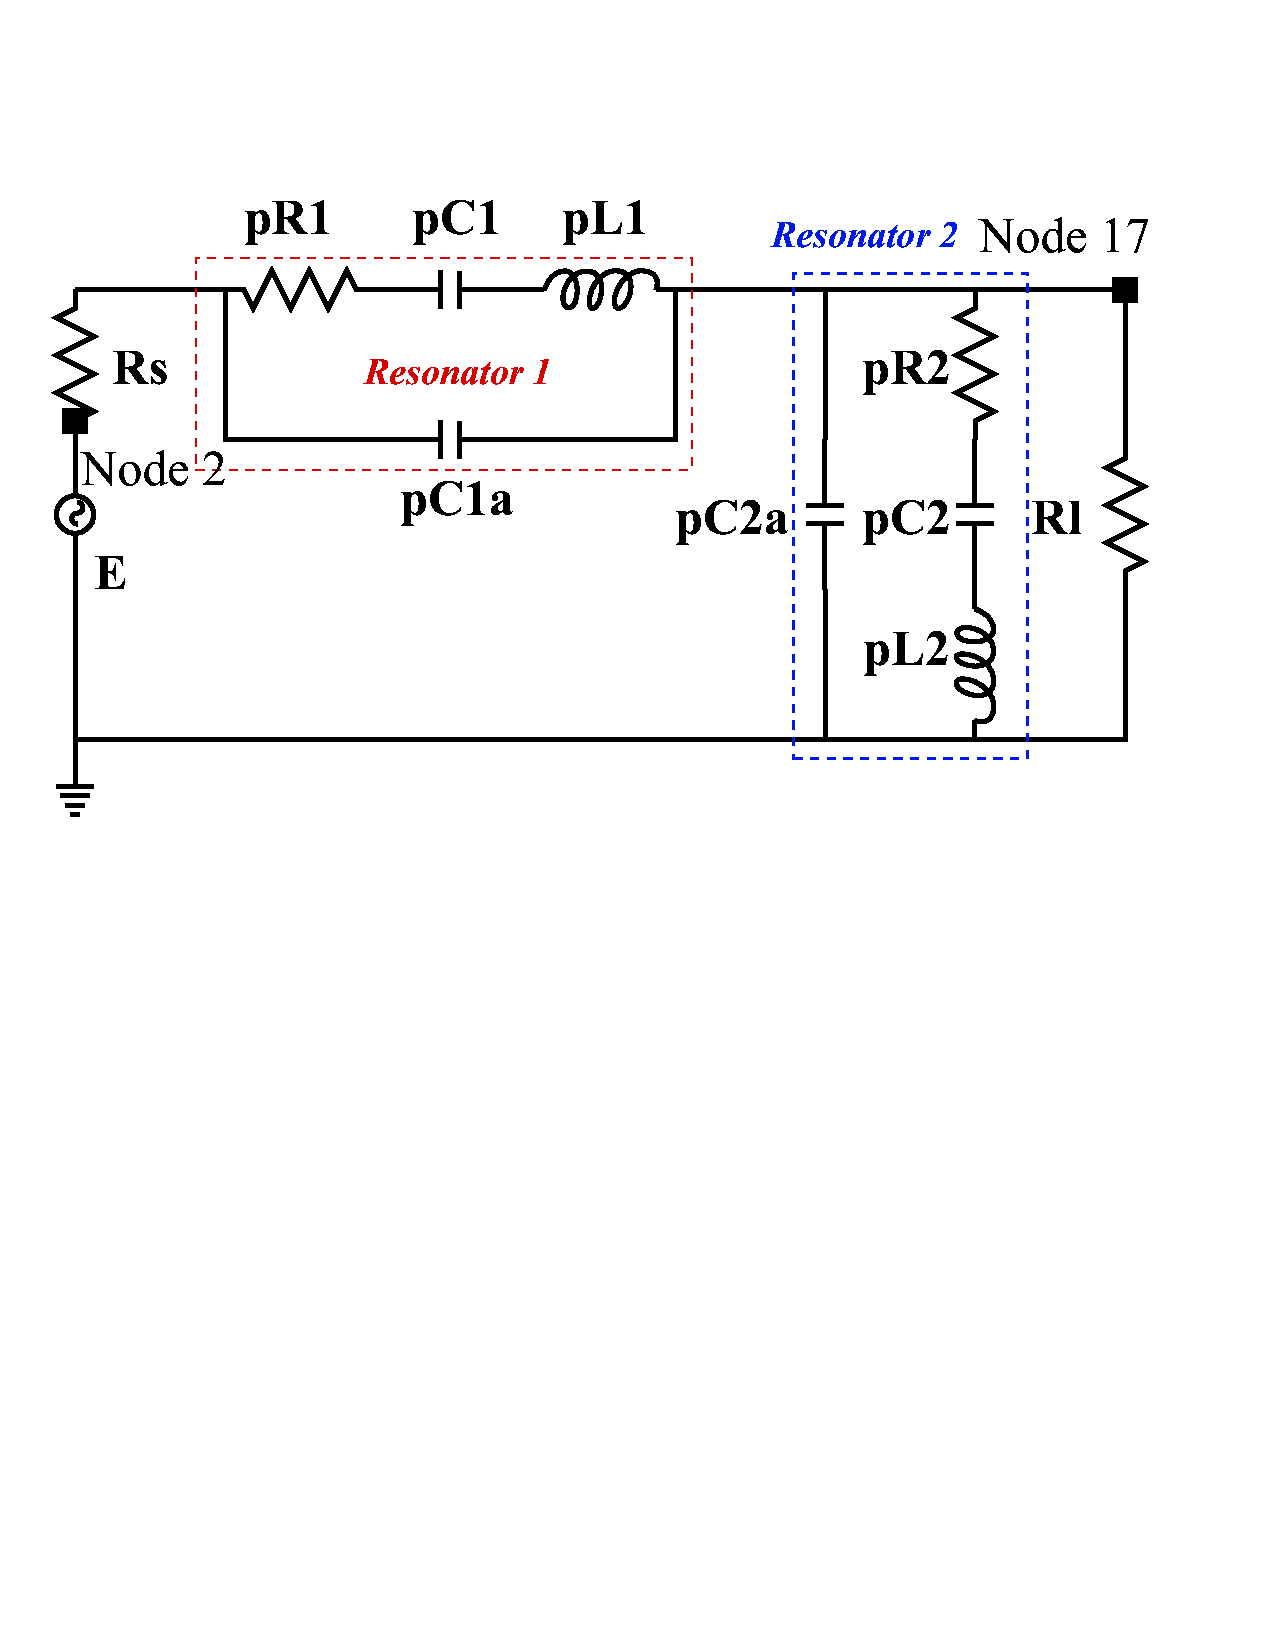
\includegraphics[trim = 0in 5in 0in 0in, clip, height = 3in]{fig/ladderfilter.pdf}
\caption{Schematic of the Ladder filter}
\label{fig:LadderFilter}
\end{figure}

\clearpage
\subsubsection*{Input file (LUA)}
\begin{flushleft}
  \textbf{Inputfile:}
  \ttt{\ttilde/hiqlab/models/tutorial/circuit\_test/ladder\_filter.lua}\\
\end{flushleft}
\hspace{1in}
{\footnotesize
\listinginput[10]{1}{../../../models/tutorial/circuit_test/ladder_filter.lua}
}

\clearpage
Only the portions emphasized are explained in detail.

\begin{itemize}

  \item{\textbf{Define circuit elements:}}
  The flags \ttt{insert1} and \ttt{insert2} allow 
  one to select which filters are included in the circuit.
  The material properties of the lumped LRC components can
  also be complex, in which case a table with the real and
  imaginary parts are passed to the \ttt{make\_material\_LRC}
  constructor. The element number of the \ttt{wire} added between
  nodes 1 and 2 have been returned since an element variable driving 
  condition will be added for the ac voltage source.

  \item{\textbf{Define nodal boundary condition:}}
  The nodes which are grounded are specified.

  \item{\textbf{Define driving and sensing functions:}}
  The circuit is driven with an AC voltage source defined 
  through an element variable driving condition on the 
  \ttt{wire} element by the function \ttt{ac\_voltage\_source}. 
  If the index of the
  element \ttt{ind} equals the element number \ttt{elem1} of
  the wire, a value of \ttt{E} is specfied as the voltage
  difference between the nodes that \ttt{wire} is connected to. 

  The voltages at node 3 an 17 are sensed. 

\end{itemize}

\clearpage
\subsubsection*{Solve for transfer function (MATLAB)}
\begin{flushleft}
  \textbf{Inputfile:}
  \ttt{\ttilde/hiqlab/models/tutorial/circuit\_test/ladder\_filter.m}\\
\end{flushleft}
\hspace{1in}
{\footnotesize
\listinginput[10]{1}{../../../models/tutorial/circuit_test/ladder_filter.m}
}

\clearpage
The steps to compute the transfer function of the low pass
filter are explained here. 

\begin{itemize}

  \item{\textbf{Get driving and sensing patterns:}}
  The sensing patterns for the voltages at node 3 and 4
  are obtained by the function \ttt{Mesh\_get\_sense\_u}
  which in turn look for the appropriate functions in the
  Lua input file. Since the driving pattern is obtained
  by the contribution that comes from an element variable
  in \ttt{wire} defined by the Lua function
  \ttt{ac\_voltage\_source}, it must be called by
  \ttt{Mesh\_get\_drive\_elements\_f}.

  \item{\textbf{Compute transfer function:}}
  Though this is a first
  order problem the function second order bode can be
  called for transfer function evaluation, but the
  option  \ttt{mkc} must be set to 1 to include the
  \ttt{C} matrix.

  \item{\textbf{Compute analytical result:}}
  For this case the analytical result is computed.

\end{itemize}

\begin{figure}[htbp]
\centering
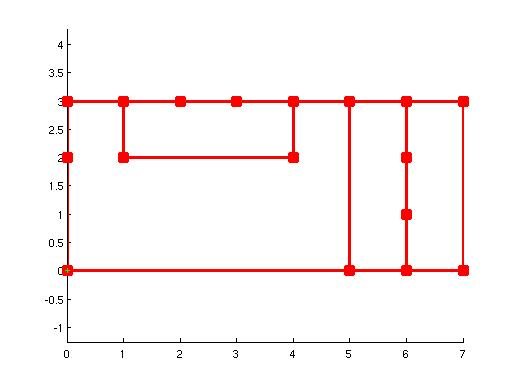
\includegraphics[height = 3in]{fig/ladder_filter_mesh.jpg}
\caption{Mesh for a Ladder filter}
\label{fig:LadderFilterMesh}
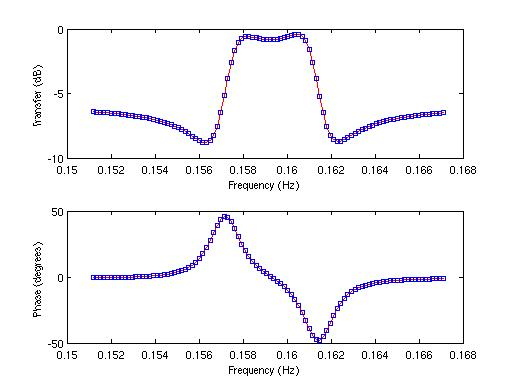
\includegraphics[height = 3in]{fig/ladder_filter_transfer.jpg}
\caption{Transfer function  for a Ladder filter}
\label{fig:LadderFilterTransfer}
\end{figure}

\clearpage
\subsection{Electrostatic parallel plate capacitor}
\begin{flushleft}
  \textbf{Inputfile:}
  \ttt{\ttilde/hiqlab/models/tutorial/e\_pp\_capacitor}\\
  \textbf{Lua functions used:}
\end{flushleft}

\begin{figure}[htbp]
\begin{minipage}{0.3\linewidth}
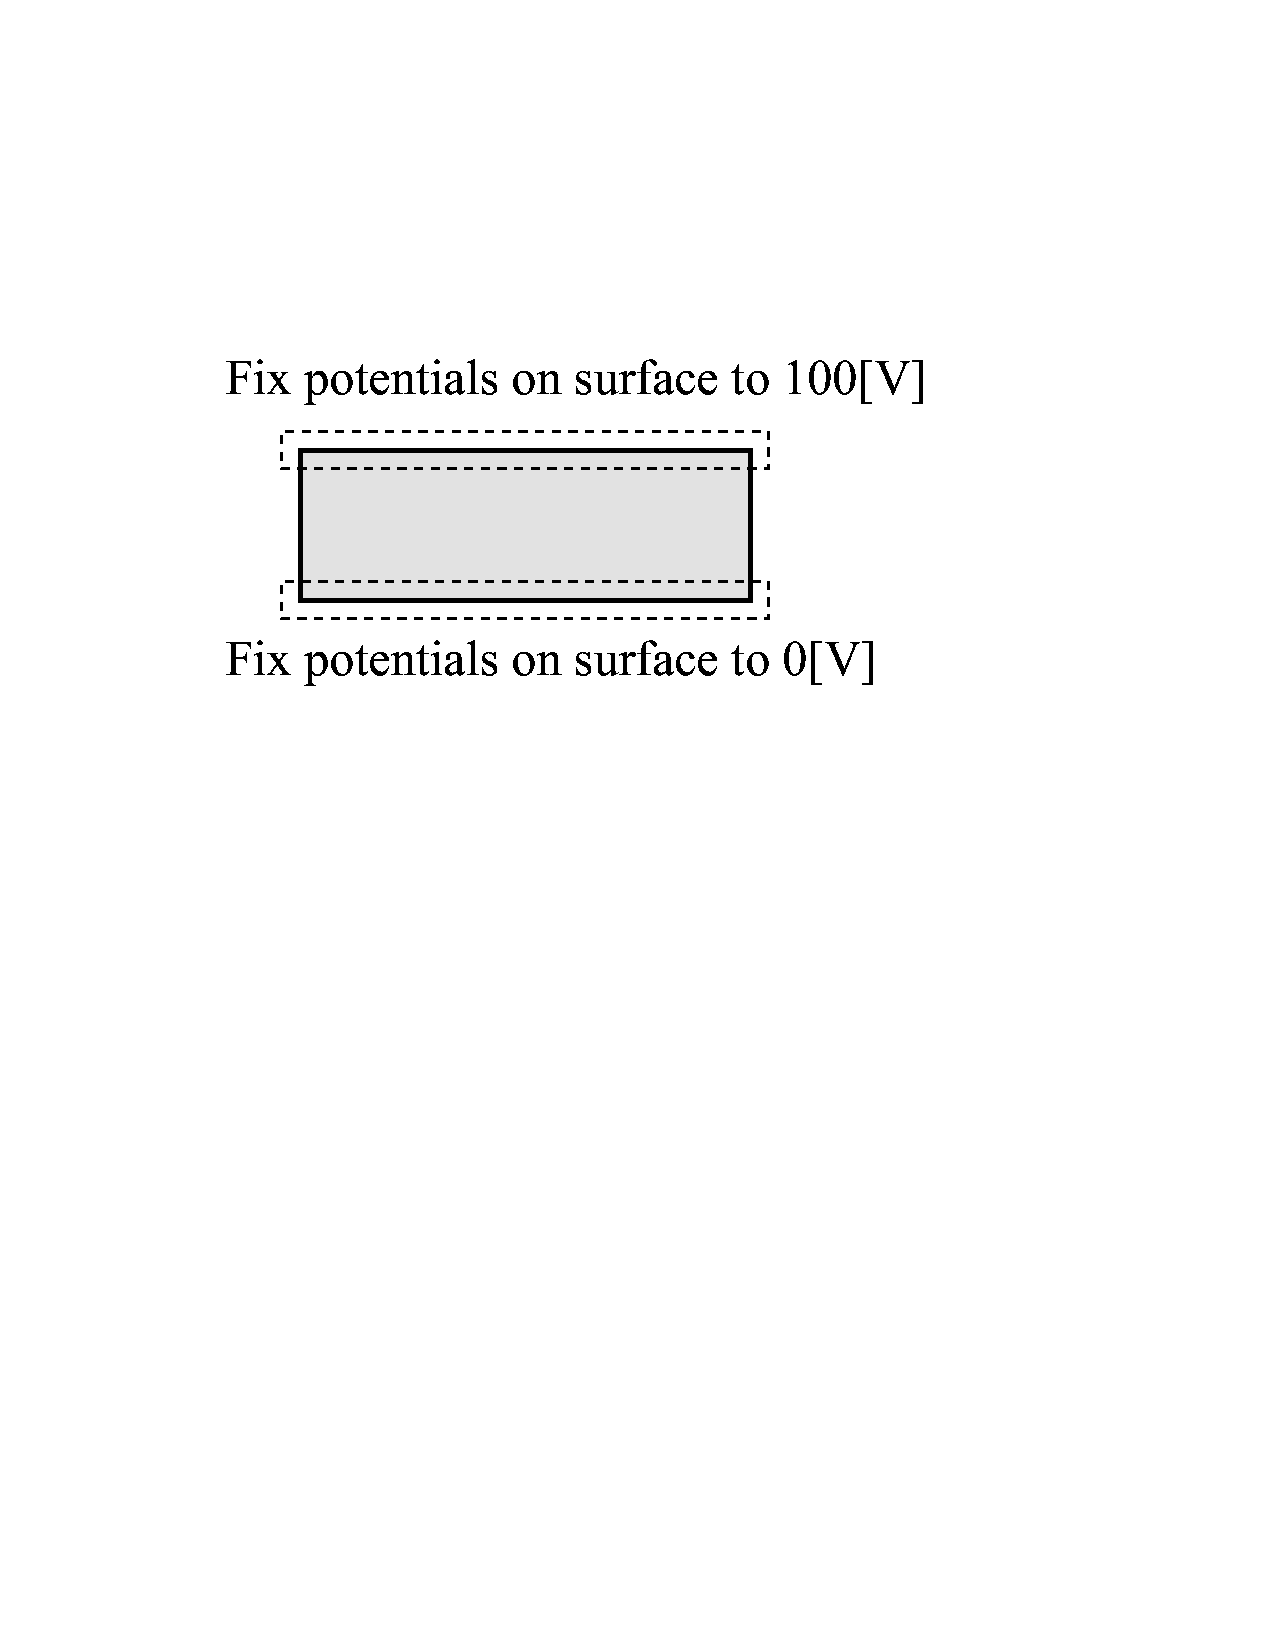
\includegraphics[trim = 1in 4.5in 2in 0.5in, clip, height = 2.5in]{fig/e_capacitor_fix.pdf}
\caption{Capacitor with fixed boundary conditions on potentials}
\end{minipage}
\hfill
\begin{minipage}{0.3\linewidth}
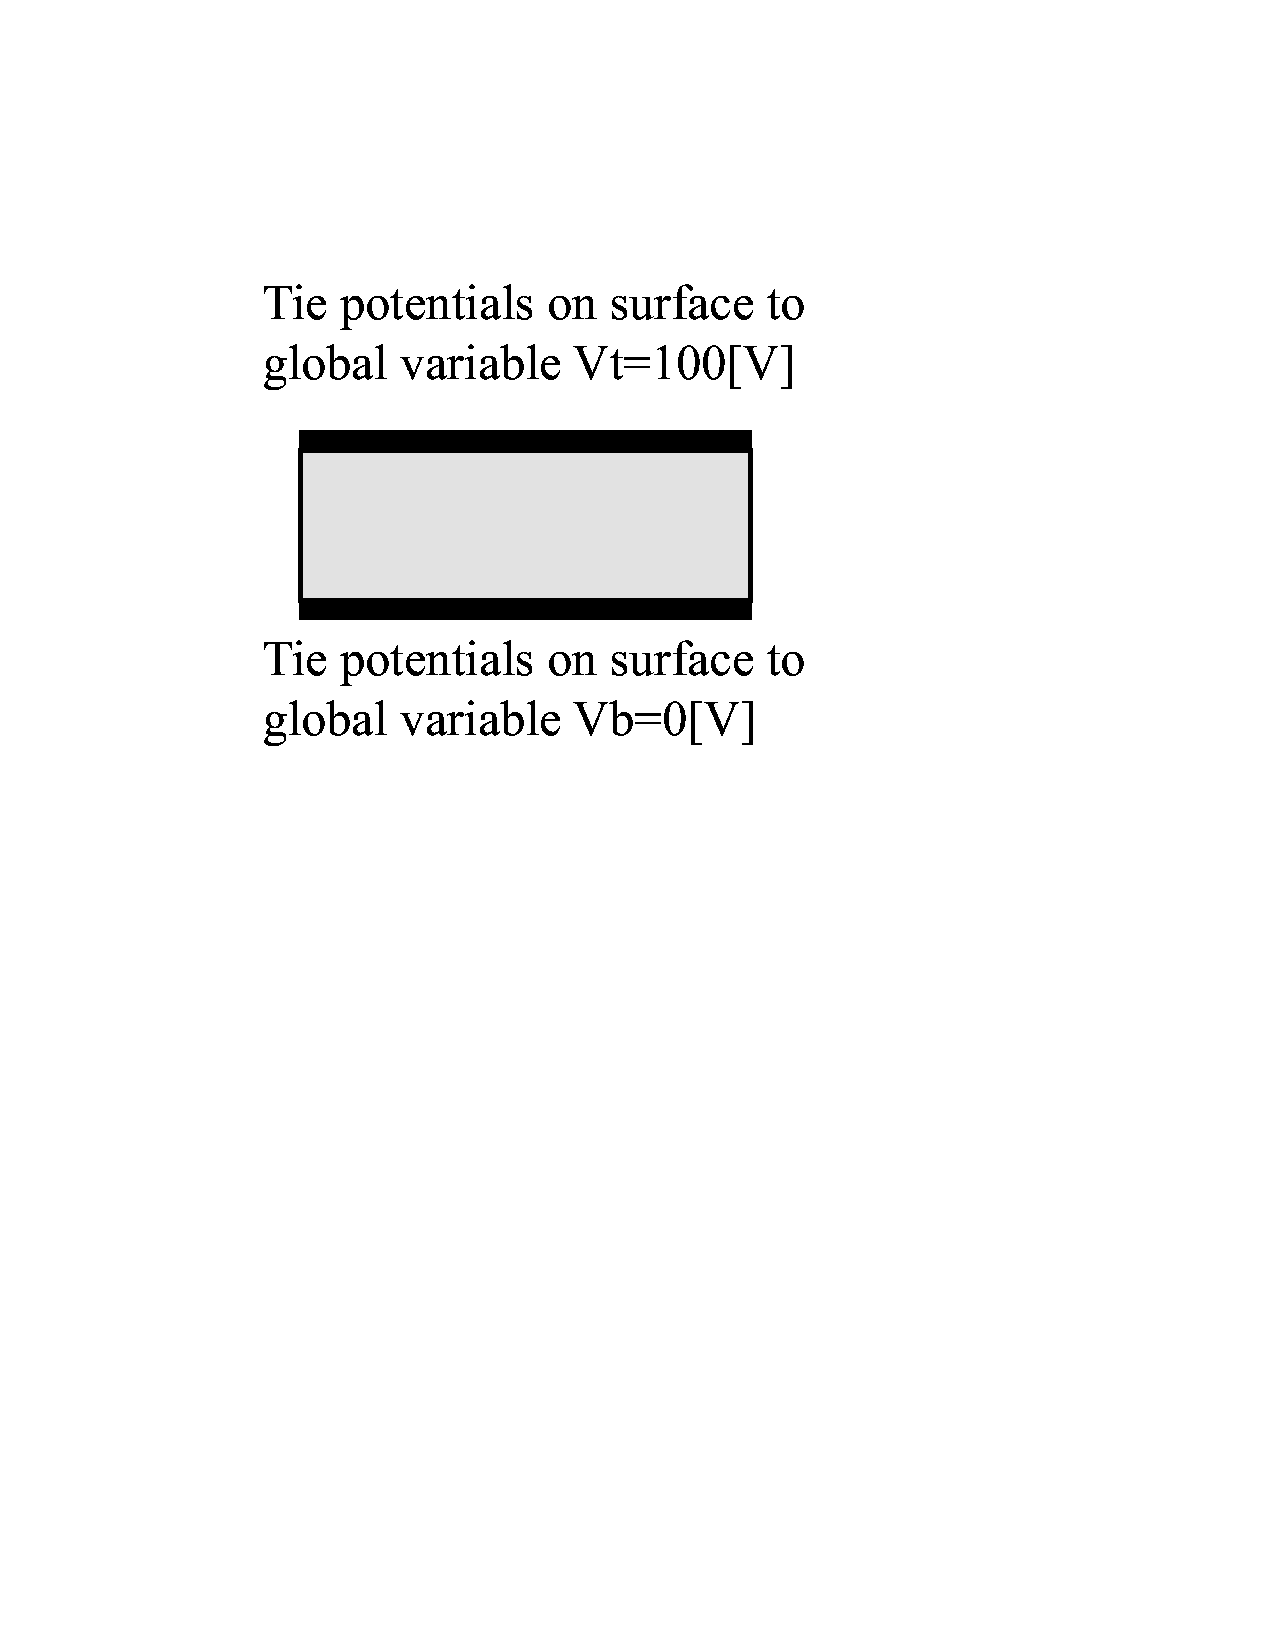
\includegraphics[trim = 1in 4.5in 2in 0.5in, clip, height = 2.5in]{fig/e_capacitor_globals.pdf}
\caption{Capacitor with potentials fixed to global variables}
\end{minipage}
\hfill
\begin{minipage}{0.3\linewidth}
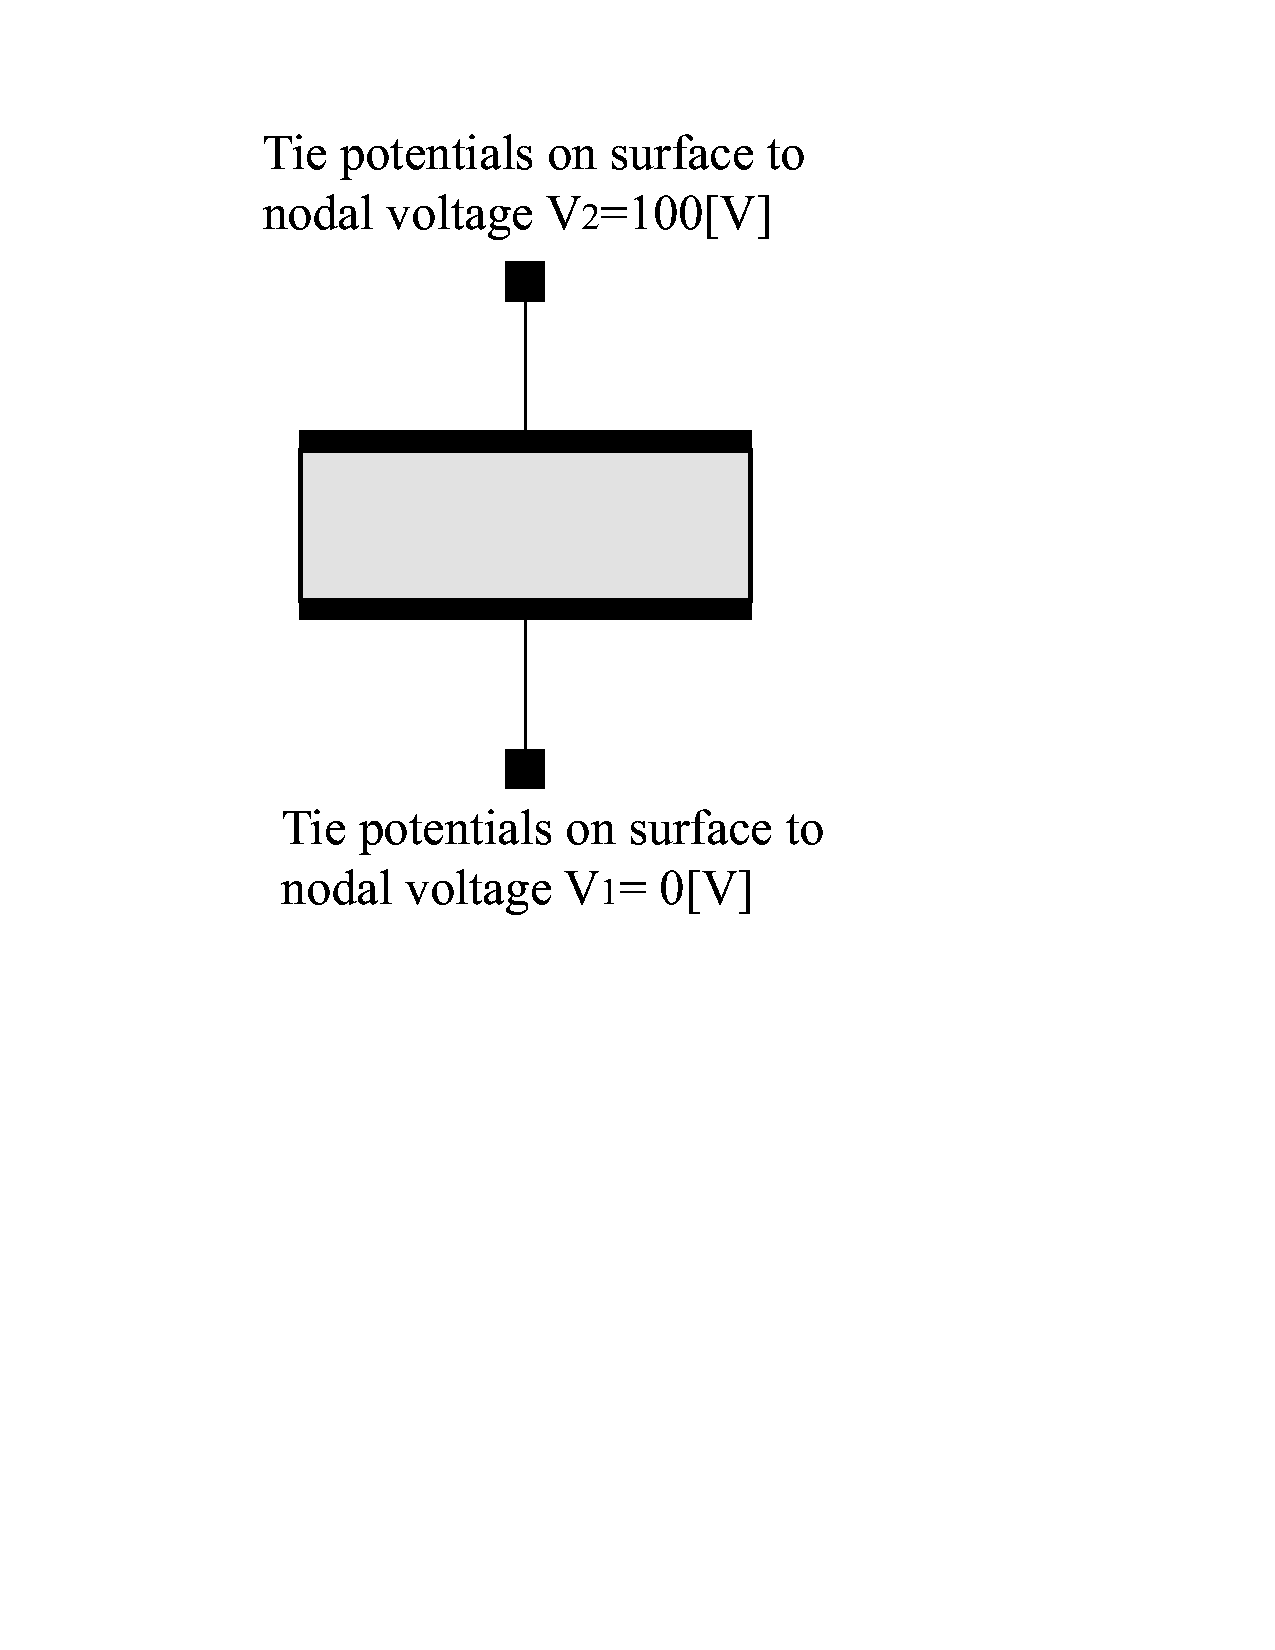
\includegraphics[trim = 1in 4.5in 2in 0.5in, clip, height = 2.5in]{fig/e_capacitor_electrodes.pdf}
\caption{Capacitor with potentials fixed to nodal volatage}
\end{minipage}
\end{figure}

\clearpage
\subsubsection*{Input file (LUA)}
\begin{flushleft}
  \textbf{Inputfile:}
  \ttt{\ttilde/hiqlab/models/tutorial/e\_pp\_capacitor/e\_pp\_capacitor2d.lua}\\
\end{flushleft}
\hspace{1in}
{\footnotesize
\listinginput[10]{1}{../../../models/tutorial/e_pp_capacitor/e_pp_capacitor2d.lua}
}

\clearpage
Only the portions emphasized are explained in detail.

\begin{itemize}

  \item{\textbf{Define element type:}}
  Constuct an electrostatic element with the constructor
  \ttt{make\_material\_electrostatic} where the first 
  argument specifies the permitivity of the element.

  \item{\textbf{Set boundary condition:}}
  If no string is set to \ttt{use\_case} then
  nodal boundary conditions are set to the top and bottom
  potential variables. 

  If \ttt{use\_case=='eppc2d\_using\_globals\_sta.lua'}, then
  the file \ttt{eppc2d\_using\_globals\_sta.lua} is loaded.
  The file is shown in Figure 
  \ref{fig:LuaInputFile:eppc2d_using_globals_sta.lua}.
  \begin{itemize}

     \item{\textbf{Define global shape functions:}}
     Two global shape functions are defined for the two global
     variables.

     \item{\textbf{Add global variables:}}
     The two global variables are added by the \ttt{mesh:add\_global} 
     command. The first argument specifies the function associated with 
     the global variable. The second and third arguments are 
     the values that are used to non-dimensionalize the primary
     and secondary variable. Since we would like to define
     boundary conditions on these global variables, the number of
     the global variable must be stored in \ttt{idg\_t,idg\_b}. 

     \item{\textbf{Define global variable boundary condtion function:}}
     A function with the global variable number as the input 
     argument is defined to specify global variable boundary 
     conditions. When the number \ttt{idg} is equal to the 
     \ttt{idg\_t}, the global variable number associated with the top
     electrode, a value of \ttt{Vf\_dc} is assigned. 
     When the number \ttt{idg} is equal to the 
     \ttt{idg\_b}, the global variable number associated with the 
     bottom electrode, a value of zero is assigned. 

     \item{\textbf{Set global variables:}}
     Once the global variables are added to the mesh they must
     be set by the \ttt{mesh:set\_globals()} command. 

     \item{\textbf{Set global variable boundary conditions:}}
     The global variable boundary condition is set by the command
     \ttt{mesh:set\_globals\_bc}.

  \end{itemize}

  If \ttt{use\_case=='eppc2d\_using\_electrodes\_sta.lua'}, then
  the file \ttt{eppc2d\_using\_electrodes\_sta.lua} is loaded.
  The file is shown in Figure 
  \ref{fig:LuaInputFile:eppc2d_using_electrodes_sta.lua}.
  \begin{itemize}

     \item{\textbf{Add nodes:}}
     To use the electrode element they must connected to nodes 
     with voltage variables. These nodes are added in these lines
     of code.

     \item{\textbf{Define global shape functions:}}
     Two global shape functions are defined for the two global
     variables that are incorporated in the electrode element.

     \item{\textbf{Add electrode element:}}
     The electrode element is added by the function
     \ttt{add\_electrode}. The first argument specifies the 
     type of electrode used. The second argument specifies the 
     number of node that the electrode is connected to. The
     third specifies the global variable shape function that
     is used to tie the potential variables to the voltage variable
     of the node. The last argument is an optional scaling parameter
     to account for the 2D analysis.(See section on electrode for
     details). This constructor can return the element number of 
     the electrode element (\ttt{eno\_d,eno\_s}) and the global 
     variable number of the global variable (\ttt{idg\_d,idg\_s}). 
     These should be stored for reference, since they are requred
     for modal computation and equivalent circuit parameter 
     extraction. 

     \item{\textbf{Define nodal boundary condition:}}
     One node is specified to have voltage of \ttt{Vf\_dc}
     and the other is zero. The boundary condition for the 
     voltages are specified in the second slot since the 
     first slot is specified for the potential variables. These
     are distinguished since the dual variable for potentials 
     are defined as the charge, and the dual variable for the
     voltages are the currents. Since elements connecting 
     potential variables were added first the potentials are
     specified in the first slot.   

     \item{\textbf{Element variable sensing functions:}}
     For the electrode element, the global variable pertains
     to the element and can be accessed also as an element 
     variable. For the electrode element the first element 
     variable accesses this global variable which is the 
     voltage. The second element variable is the total charge.

     These can are sensed by the functions defined here.

     \item{\textbf{Set global variables:}}
     Once the global variables are added to the mesh they must
     be set by the \ttt{mesh:set\_globals()} command. 

     \item{\textbf{Set global variable boundary conditions:}}
     The global variable boundary condition is set by the command
     \ttt{mesh:set\_globals\_bc}.

  \end{itemize}

  \item{\textbf{Nodal variable sensing functions:}}
  The function \ttt{sense\_top\_Q} is used to sense the potentials
  on the top electrode and \ttt{sense\_bot\_Q} for the bottom.
 
\end{itemize}

\clearpage
\begin{figure}[htbp]
  {\footnotesize
  \listinginput[10]{1}{../../../models/tutorial/e_pp_capacitor/eppc2d_using_globals_sta.lua}
  }
  \caption{Lua input file for an electrostatic parallel plate
   capacitor using globals (\ttt{eppc2d\_using\_globals\_sta.lua})}
  \label{fig:LuaInputFile:eppc2d_using_globals_sta.lua}
\end{figure}

\begin{figure}[htbp]
  {\footnotesize
  \listinginput[10]{1}{../../../models/tutorial/e_pp_capacitor/eppc2d_using_electrodes_sta.lua}
  }
  \caption{Lua input file for an electrostatic parallel plate
capacitor using electrodes (\ttt{eppc2d\_using\_electrodes\_sta.lua})}
  \label{fig:LuaInputFile:eppc2d_using_electrodes_sta.lua}
\end{figure}

\clearpage
\subsubsection*{Solve electrostatic problem (MATLAB)}
\begin{flushleft}
  \textbf{Inputfile:}
  \ttt{\ttilde/hiqlab/models/tutorial/e\_pp\_capacitor/e\_pp\_capacitor2d\_sta.m}\\
\end{flushleft}
\hspace{1in}
{\footnotesize
\listinginput[10]{1}{../../../models/tutorial/e_pp_capacitor/e_pp_capacitor2d_sta.m}
}

\clearpage
The steps to compute the static state of an electrostatic 
parallel plate capacitor are 
explained here. 

\begin{itemize}

  \item{\textbf{Parameters:}}
  Select which case to use.

  \item{\textbf{Analytical solution:}}
  Extract numerical parameters from the Lua environment through the 
  function \ttt{Lua\_get\_double}, and compute the capacitance
  from the formula for a parallel plate capacitor.

  \item{\textbf{Find top and bottom charge from sensing nodal values:}}
  \ttt{Mesh\_get\_force} extracts the forces that result at the 
  nodal degrees of freedom. \ttt{force1} is a \ttt{ndf}-by-\ttt{numnp}
  array. In this case \ttt{ndf} is 1 or 2 if you use the electrode 
  element. \ttt{Mesh\_get\_sense\_force} returns the sensing vector
  for the Lua function in the \ttt{ndf}-by-\ttt{numnp} format. 
  These are contracted to obtain the charge. This charge is in
  units of Coulomb's per unit normalized length due to the plane
  assumption. Thus if we assume that the capacitor has a \ttt{Ct}
  thickness in the $z$ direction, the charge must be multiplied
  by \ttt{Ct}/\ttt{cL}, which is done to compute the capacitance.
  The normalized scale for length is obtained from the mesh through
  \ttt{Mesh\_get\_scale}.

  \item{\textbf{Find top and bottom charge from sensing free dofs:}}
  In the case that electrods are present, the total charge on the
  top and bottom of the electrode can be obtained through the 
  element variable. These are sensed by the call to 
  \ttt{Mesh\_get\_sense\_elements\_u}. Contracting this sense vector
  with the noramlized displacement vector yields the charge in 
  dimensional form. This charge is in
  units of Coulomb's per unit normalized length due to the plane
  assumption. Thus if we assume that the capacitor has a \ttt{Ct}
  thickness in the $z$ direction, the charge must be multiplied
  by \ttt{Ct}/\ttt{cL}, which is done to compute the capacitance.
  The normalized scale for length is obtained from the mesh through
  \ttt{Mesh\_get\_scale}.

\end{itemize}

Computed values for capacitance are,
\begin{verbatim}
Analytic capacitance:1.062503e-14
Computed capacitance:1.062503e-14
\end{verbatim}


\begin{figure}[htbp]
\centering
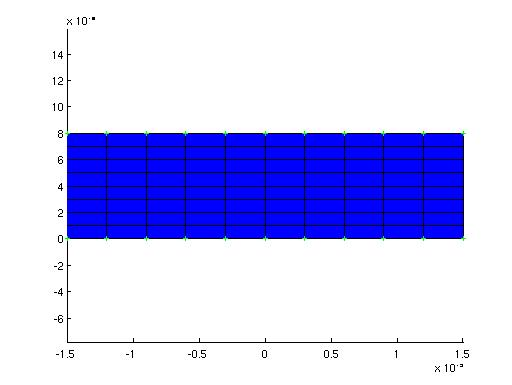
\includegraphics[height = 2in]{fig/e_pp_capacitor_mesh_fix.jpg}
\caption{Mesh for a Parallel plate capacitor using fixed boundary conditions
         on potentials or global variables}
\label{fig:ElectrostaticParallelPlateCapacitorFixMesh}
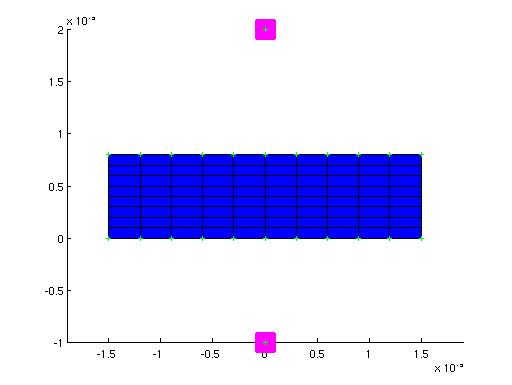
\includegraphics[height = 2in]{fig/e_pp_capacitor_mesh_electrodes.jpg}
\caption{Mesh for a Parallel plate capacitor using electrodes}
\label{fig:ElectrostaticParallelPlateCapacitorElectrodesMesh}
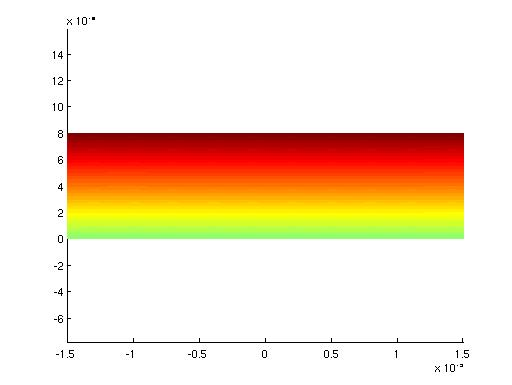
\includegraphics[height = 2in]{fig/e_pp_capacitor_field.jpg}
\caption{Potential field for a Parallel plate capacitor}
\label{fig:ElectrostaticParallelPlateCapacitorPotentialField}
\end{figure}

\clearpage
\subsection{Electromechanical parallel plate capacitor}
\begin{flushleft}
  \textbf{Inputfile:}
  \ttt{\ttilde/hiqlab/models/developing/em\_pp\_capacitor}\\
  \textbf{Lua functions used:}
\end{flushleft}

\begin{figure}[htbp]
\centering
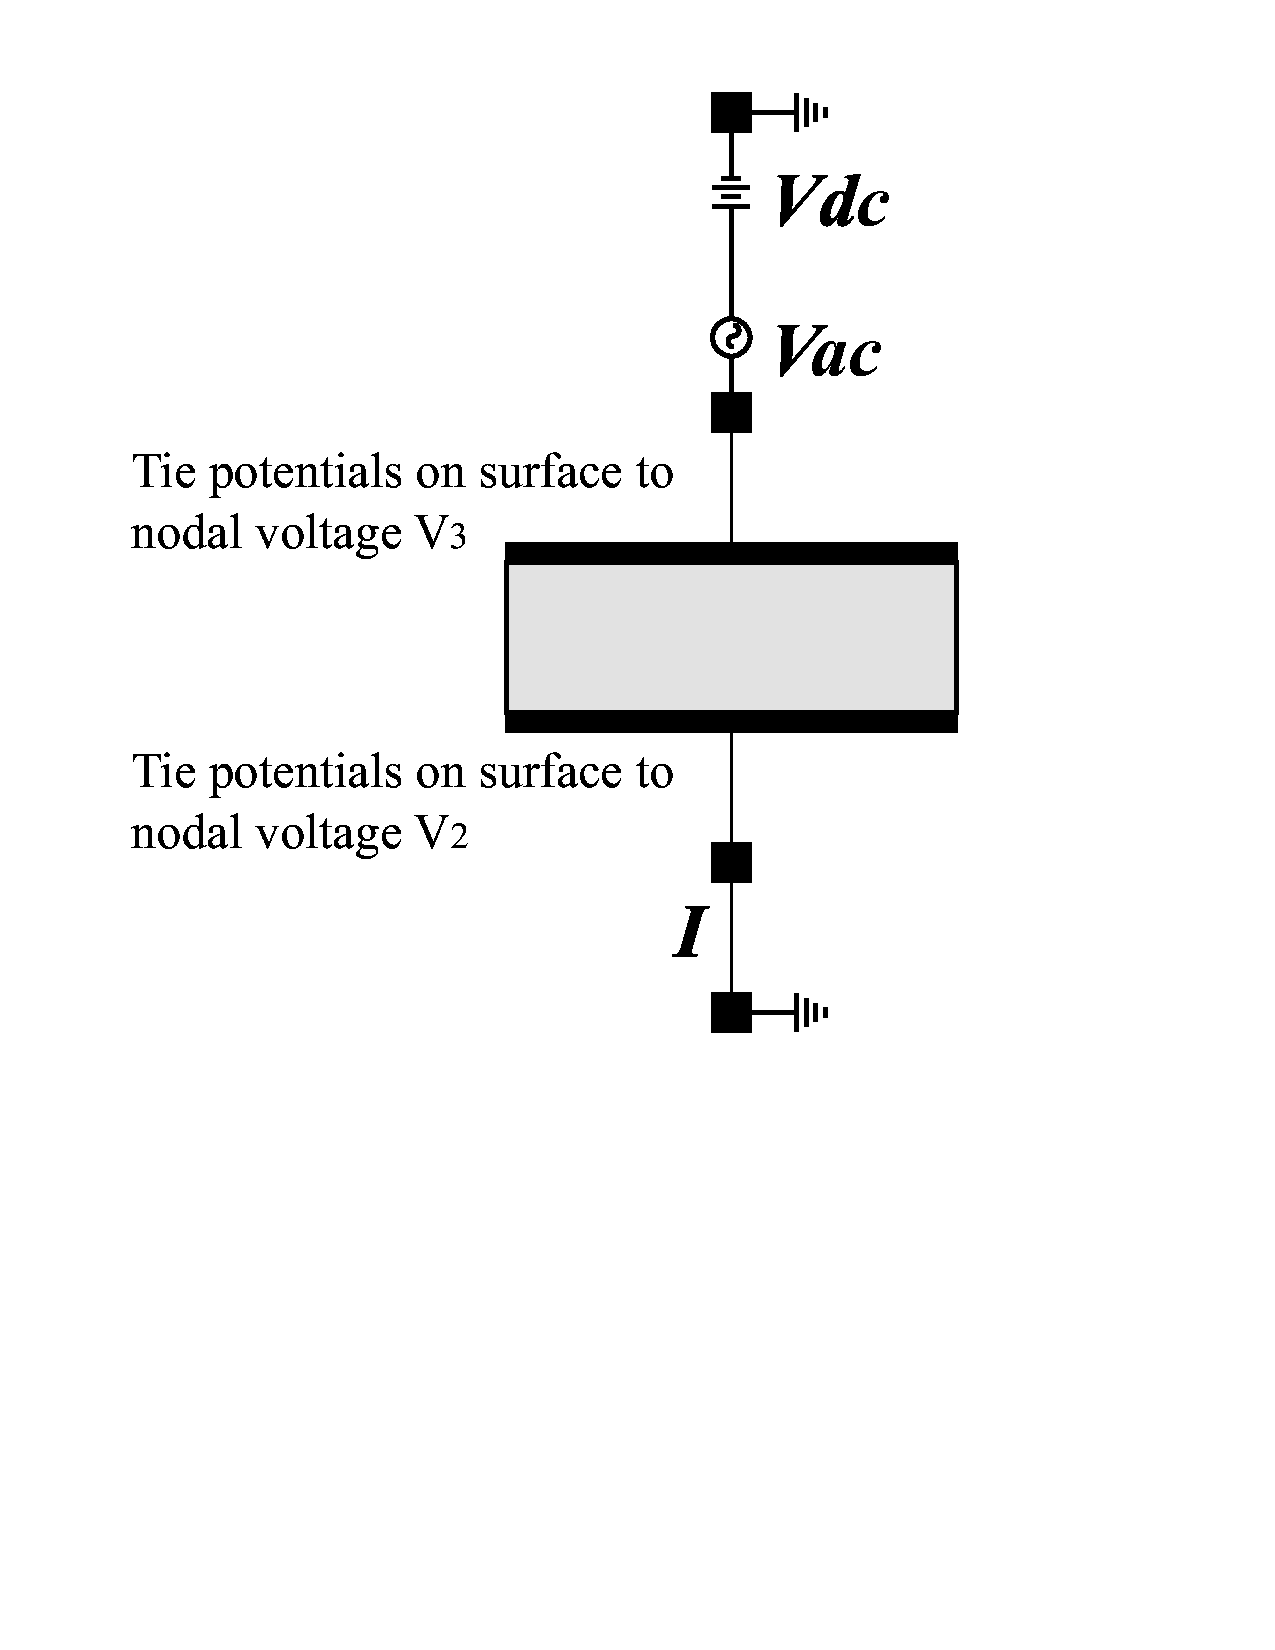
\includegraphics[trim = 1in 3.5in 2in 0.5in, clip, height = 2.5in]{fig/em_capacitor.pdf}
\caption{Electromechanical Capacitor}
\end{figure}

\clearpage
\subsubsection*{Input file (LUA)}
\begin{flushleft}
  \textbf{Inputfile:}
  \ttt{\ttilde/hiqlab/models/tutorial/em\_pp\_capacitor/em\_pp\_capacitor2d.lua}\\
\end{flushleft}
\hspace{1in}
{\footnotesize
\listinginput[10]{1}{../../../models/tutorial/em_pp_capacitor/em_pp_capacitor2d.lua}
}

\clearpage
Only the portions emphasized are explained in detail.

\begin{itemize}

  \item{\textbf{Define nondimensionalization parameters:}}
  The problem should be nondimensionalized due to the coupling
  between the mechanical and electrical domain. The characteristic
  parameters are defined by the material \ttt{silicon2} and the 
  length scale \ttt{2e-6} through the function \ttt{em\_nondim}.

  \item{\textbf{Define element type:}}
  The electromechanical coupling effect is produced by 
  constructing an element through the \ttt{make\_material\_couple\_em},
  which takes in as a first argument the permitivity, and the second
  as the type of analysis.

  \item{\textbf{Mesh center block:}}
  Additional to the elastic element, the electromechanical 
  coupling element is overlayed on top of this.

  \item{\textbf{Define mechanical boundary condition:}}
  The mechanical boundary condition is set here. The parallel
  plate capacitor will be fixed at the bottom and free at the
  top.

  \item{\textbf{Set boundary condition:}}
  The file \ttt{emppc2d\_using\_electrodes.lua} containing
  the information about electrodes and circuitry is loaded.
  \begin{itemize}

     \item{\textbf{Add nodes:}}
     To use the electrode element they must connected to nodes 
     with voltage variables. Nodes to add the voltage source is 
     also required. These nodes are added in these lines
     of code.

     \item{\textbf{Define global shape functions:}}
     Two global shape functions are defined for the two global
     variables that are incorporated in the electrode element.
     The function returns four numbers for each nodal point 
     evaluated. The first two correspond to the x and y displacements,
     the third to the nodal potentials, and the last to the nodal
     voltages. In this case the nodal potentials are all tied 
     together.

     \item{\textbf{Add discrete elements:}}
     The \ttt{wire} element is constructed and added. The
     element with element number \ttt{eno\_vd} is used
     for the voltage source. and \ttt{eno\_vs} is used
     to sense the throughput motional current.

     \item{\textbf{Add electrode element:}}
     The electrode element is added by the function
     \ttt{add\_electrode}. The first argument specifies the 
     type of electrode used. The second argument specifies the 
     number of node that the electrode is connected to. The
     third specifies the global variable shape function that
     is used to tie the potential variables to the voltage variable
     of the node. The last argument is an optional scaling parameter
     to account for the 2D analysis.(See section on electrode for
     details). This constructor can return the element number of 
     the electrode element (\ttt{eno\_d,eno\_s}) and the global 
     variable number of the global variable (\ttt{idg\_d,idg\_s}). 
     These should be stored for reference, since they are requred
     for modal computation and equivalent circuit parameter 
     extraction. 

     \item{\textbf{Nodal boundary conditions:}}
     The nodes specifying ground are defined.

     \item{\textbf{Element boundary conditions:}}
     The dc voltage source is 
     defined as an element variable boundary condition.
     It is placed at the \ttt{wire} element with node 
     number \ttt{eno\_vd}. 

     \item{\textbf{Element sensing and driving conditions:}}
     The ac voltage source is 
     defined as an element variable driving function.
     It is placed at the \ttt{wire} element with node 
     number \ttt{eno\_vd}. 

     The resulting motional current is sensed at the other
     \ttt{wire} element on the other side of the device with
     element number \ttt{eno\_vs}.

  \end{itemize}
  
  The global variables added must be set by \ttt{mesh:set\_globals()}.
  The element boundary condition for the dc voltage source is 
  set by \ttt{mesh:set\_elements\_bc}.

\end{itemize}

\clearpage
\subsubsection*{Solve static problem (MATLAB)}
\begin{flushleft}
  \textbf{Inputfile:}
  \ttt{\ttilde/hiqlab/models/tutorial/em\_pp\_capacitor/em\_pp\_capacitor2d\_sta.m}\\
\end{flushleft}
\hspace{1in}
{\footnotesize
\listinginput[10]{1}{../../../models/tutorial/em_pp_capacitor/em_pp_capacitor2d_sta.m}
}

\clearpage
The steps to compute the static response of an electromechanical
parallel plate capacitor are 
explained here. 

\begin{itemize}

  \item{\textbf{Compute for static case:}}
  Since the electromechanical coupling effect is nonlinear,
  a nonlinear solution method must be used. By giving an 
  option \ttt{nonlinear} specifying the method of choice to
  \ttt{static\_state}, this can be done. \ttt{'NR'} uses
  Newton-Raphson.

  \item{\textbf{Analytical solution:}}
  Extract numerical parameters from the Lua environment through the 
  function \ttt{Lua\_get\_double}, and compute the capacitance
  from the formula for a parallel plate capacitor.
  
  \item{\textbf{Find top and bottom charge from sensing free dofs:}}
  In the case that electrods are present, the total charge on the
  top and bottom of the electrode can be obtained through the 
  element variable. These are sensed by the call to 
  \ttt{Mesh\_get\_sense\_elements\_u}. Contracting this sense vector
  with the noramlized displacement vector yields the charge in 
  dimensional form. This charge is in
  units of Coulomb's per unit normalized length due to the plane
  assumption. Thus if we assume that the capacitor has a \ttt{Ct}
  thickness in the $z$ direction, the charge must be multiplied
  by \ttt{Ct}/\ttt{cL}, which is done to compute the capacitance.
  The normalized scale for length is obtained from the mesh through
  \ttt{Mesh\_get\_scale}.

\end{itemize}

Computed values are,
\begin{verbatim}
Analytic capacitance:1.062503e-14
Computed capacitance:1.062504e-14
\end{verbatim}


\begin{figure}[htbp]
\centering
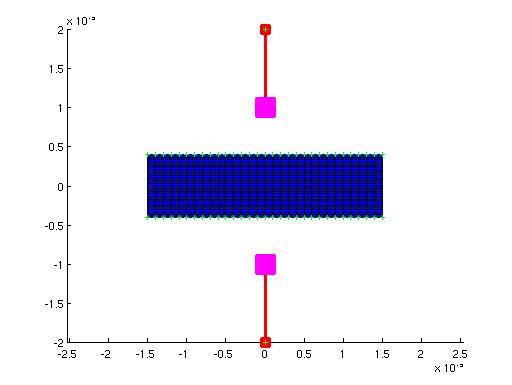
\includegraphics[height = 3in]{fig/em_pp_capacitor_mesh.jpg}
\caption{Mesh for an Electromechanical parallel plate capacitor}
\label{fig:ElectromechanicalParallelPlateCapacitorFixMesh}
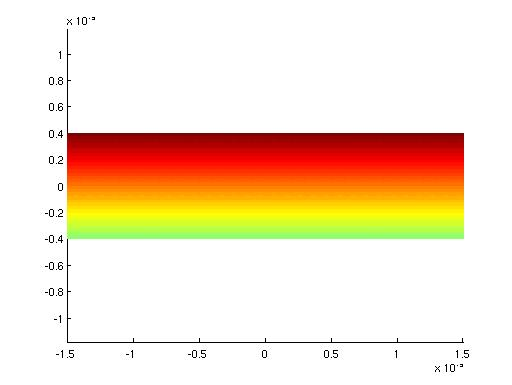
\includegraphics[height = 3in]{fig/em_pp_capacitor_field.jpg}
\caption{Potential field for an Electromechanical parallel plate capacitor}
\label{fig:ElectromechanicalParallelPlateCapacitorPotentialField}
\end{figure}

\clearpage
\subsubsection*{Solve dynamic modal problem (MATLAB)}
\begin{flushleft}
  \textbf{Inputfile:}
  \ttt{\ttilde/hiqlab/models/tutorial/em\_pp\_capacitor/em\_pp\_capacitor2d\_dyn.m}\\
\end{flushleft}
\hspace{1in}
{\footnotesize
\listinginput[10]{1}{../../../models/tutorial/em_pp_capacitor/em_pp_capacitor2d_dyn.m}
}

\clearpage
The steps to compute the modes of an electromechanical
parallel plate capacitor are 
explained here. 

\begin{itemize}

  \item{\textbf{Extract element and global numbers for electrodes:}}
  The element numbers and global variable numbers of the electrode
  elements are extracted from the Lua input file through the function
  \ttt{Lua\_get\_double} for the modal computation. The 1 is added
  since the numbers for the elements and global variables are given
  with zero indexing in the Lua environment. These are stored as an
  array in the structure \ttt{param}, under the field \ttt{eno} and
  \ttt{idg}. 

  \item{\textbf{Compute frequencies, Qs, and mode shapes:}}
  The function \ttt{emcmode} is used to compute \ttt{nev}
  modes closest to the frequence \ttt{w0}[rad/s]. 

\end{itemize}

Computed values are,
\begin{verbatim}
Freq [Hz]   :1.917998e+08
            :2.048102e-13
Q           :4.682378e+20
\end{verbatim}

\clearpage
\subsubsection*{Solve for the forced response (MATLAB)}
\begin{flushleft}
  \textbf{Inputfile:}
  \ttt{\ttilde/hiqlab/models/tutorial/em\_pp\_capacitor/em\_pp\_capacitor2d\_for.m}\\
\end{flushleft}
\hspace{1in}
{\footnotesize
\listinginput[10]{1}{../../../models/tutorial/em_pp_capacitor/em_pp_capacitor2d_for.m}
}

\clearpage
The steps to compute the forced response of an electromechanical
parallel plate capacitor are 
explained here. 

\begin{itemize}

  \item{\textbf{Construct forcing vectors, compute harmonic response:}}
  The harmonic response is computed by \ttt{harmonic\_state}. The
  option \ttt{mkc} must be set to 1, for the case when circuit nodes
  are present. 

\end{itemize}

\begin{figure}[htbp]
\centering
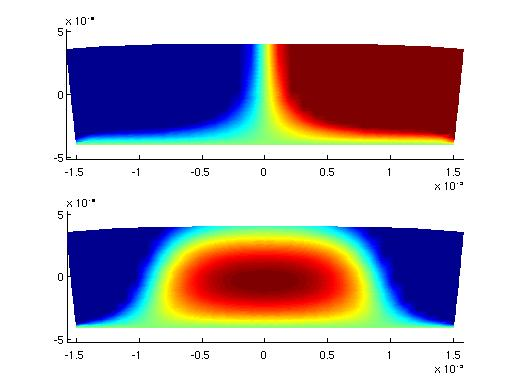
\includegraphics[height = 3in]{fig/em_pp_capacitor_mode.jpg}
\caption{Mode shape for an Electromechanical parallel plate capacitor}
\label{fig:ElectromechanicalParallelPlateCapacitorMode}
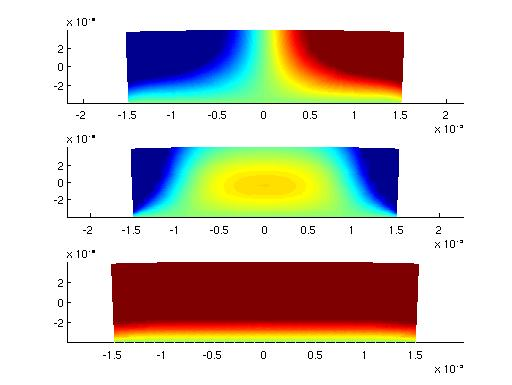
\includegraphics[height = 3in]{fig/em_pp_capacitor_forced.jpg}
\caption{Forced response for an Electromechanical parallel plate capacitor}
\label{fig:ElectromechanicalParallelPlateCapacitorForced}
\end{figure}

\clearpage
\subsubsection*{Solve for the admittance (MATLAB)}
\begin{flushleft}
  \textbf{Inputfile:}
  \ttt{\ttilde/hiqlab/models/tutorial/em\_pp\_capacitor/em\_pp\_capacitor2d\_vi.m}\\
\end{flushleft}
\hspace{1in}
{\footnotesize
\listinginput[10]{1}{../../../models/tutorial/em_pp_capacitor/em_pp_capacitor2d_vi.m}
}

\clearpage
The steps to compute the admittance of an electromechanical
parallel plate capacitor are 
explained here. 

\begin{itemize}

  \item{\textbf{Compute transfer function:}}
  The transfer function is computed by \ttt{second\_order\_bode}. The
  option \ttt{mkc} must be set to 1, for the case when circuit nodes
  are present. The admittance is obtained by dividing the obtained
  motional current by the applied ac voltage.

\end{itemize}

\clearpage
\subsubsection*{Solve for equivalent LRCC parameters (MATLAB)}
\begin{flushleft}
  \textbf{Inputfile:}
  \ttt{\ttilde/hiqlab/models/tutorial/em\_pp\_capacitor/em\_pp\_capacitor2d\_eq.m}\\
\end{flushleft}
\hspace{1in}
{\footnotesize
\listinginput[10]{1}{../../../models/tutorial/em_pp_capacitor/em_pp_capacitor2d_eq.m}
}

\clearpage
The steps to compute the equivalent LRCC parameters of an 
electromechanical parallel plate capacitor are 
explained here. 

\begin{itemize}

  \item{\textbf{Extract element and global numbers for electrodes:}}
  The element numbers and global variable numbers of the electrode
  elements are extracted from the Lua input file through the function
  \ttt{Lua\_get\_double} for the parameter computation. The 1 is added
  since the numbers for the elements and global variables are given
  with zero indexing in the Lua environment. These are stored as an
  array in the structure \ttt{param}, under the field \ttt{eno} and
  \ttt{idg}. 

  \item{\textbf{Compute equivalent paramters:}}
  The equivalent parameters are computed by the function
  \ttt{equiv\_LRCC}. The second argument \ttt{w0} defines the
  frequency at which the lumped parameters are set. 

\end{itemize}

The obtained values are,
\begin{verbatim}
L = 23.1532
R = 4.0693e-05
C = 2.9739e-20
C0 = 1.0626e-14
\end{verbatim}

\begin{figure}[htbp]
\centering
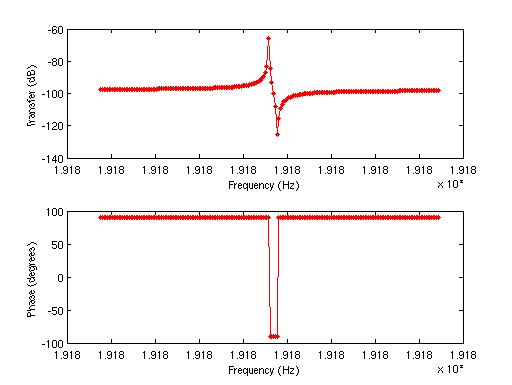
\includegraphics[height = 2.2in]{fig/em_pp_capacitor_admittance.jpg}
\caption{Admittance for an Electromechanical parallel plate capacitor}
\label{fig:ElectromechanicalParallelPlateCapacitorAdmittance}
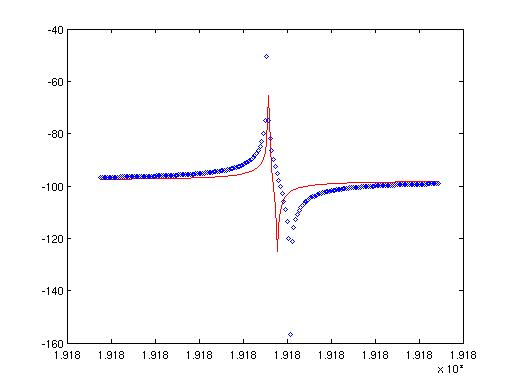
\includegraphics[height = 2.2in]{fig/em_pp_capacitor_eq_magnitude.jpg}
\caption{Magnitude of admittance for Equivalent circuit}
\label{fig:ElectromechanicalParallelPlateCapacitorEqMagnitude}
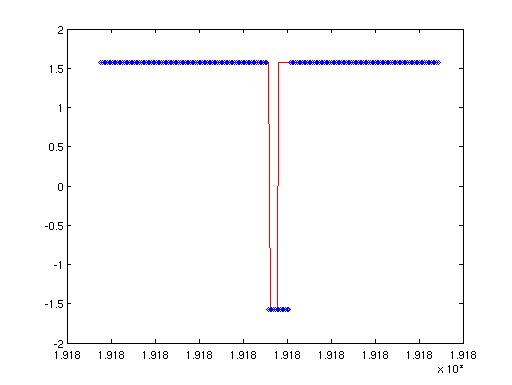
\includegraphics[height = 2.2in]{fig/em_pp_capacitor_eq_phase.jpg}
\caption{Phase of admittance for Equivalent circuit}
\label{fig:ElectromechanicalParallelPlateCapacitorEqPhase}
\end{figure}
